% =================================================================================================
% File:			client_tier.tex
% Description:	Defiinisce la sezione relativa al front-end dell'applicazione
% Created:		2015-03-27
% Author:		Tesser Paolo
% Email:		tesser.paolo@mashup-unipd.it
% =================================================================================================
% Modification History:
% Version		Modifier Date		Change											Author
% 0.0.1 		2015-03-27 			creato scheletro								Tesser Paolo
% =================================================================================================
% 0.0.2			2015-03-28			inserito scheletro del package					Tesser Paolo
% =================================================================================================
% 0.0.3			2015-04-04			inseriti padri dei package e pack contenuti		Tesser Paolo
% =================================================================================================
% 0.0.4			2015-04-04			inserite classi del package View				Tesser Paolo
% =================================================================================================
%

% CONTENUTO DEL CAPITOLO

\subsection{Client (Front-end)} % (fold)
\label{sub:client}
Nel descrivere le componenti si parlerà di classi, che però saranno da intendersi nella loro accezione logica. Il linguaggio di programmazione impiegato infatti non possiede la struttura di classe, ma solo di oggetto, sarà quindi compito del codificatore riportare le classi di seguito identificate nelle strutture fornite dallo specifico linguaggio.

	\subsubsection{client} % (fold)
	\label{ssub:bdsm_app_client}
	\begin{figure}[htbp]
		\centering
		\centerline{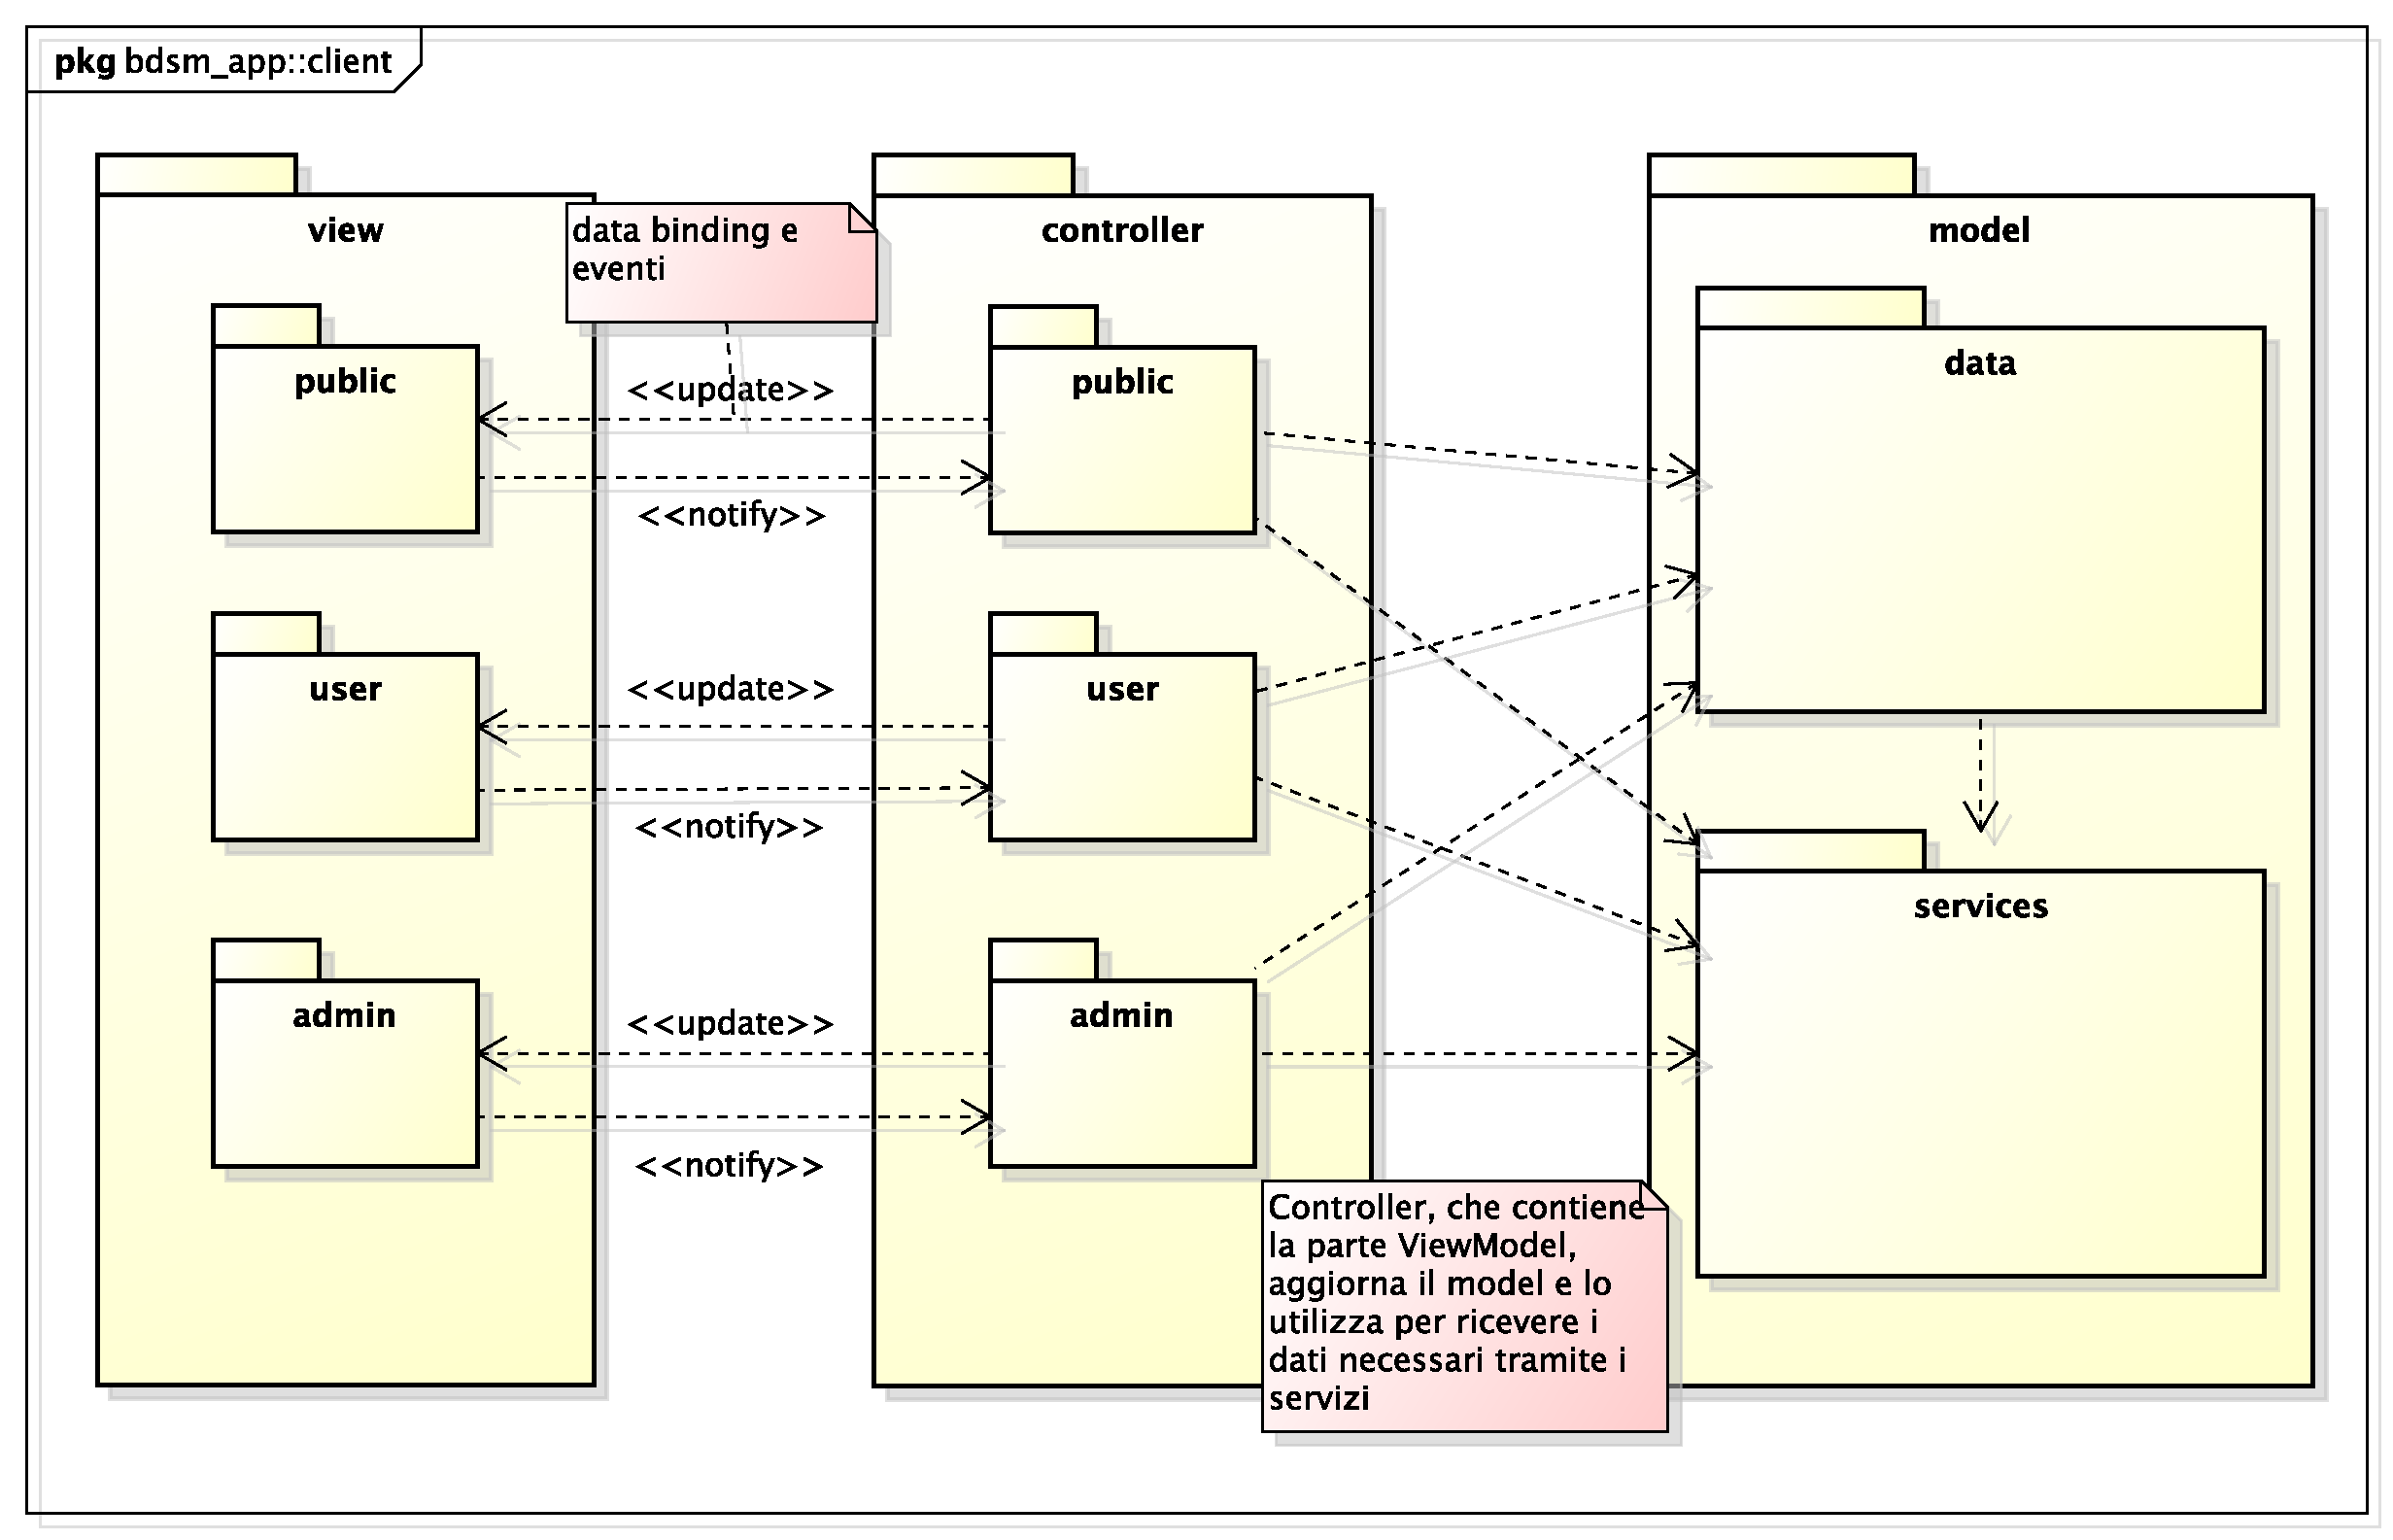
\includegraphics[scale=0.45]{./images/client/client.pdf}}
		\label{fig:package_client}
		\caption{Package - client}
	\end{figure}

	\begin{itemize}
		\item \textbf{Descrizione}: è il package che racchiude tutte le parti del front-end. \'E quindi l'insieme dei componenti che viene eseguito nel browser degli utenti normali e degli amministratori, fornendo loro un'interfaccia grafica per interagire con il sistema;
		\item \textbf{Package contenuti}:
			\begin{itemize}
				\item client::model
				\item client::view
				\item client::controller
			\end{itemize}
		\item \textbf{Interazione con altri componenti}: interagisce con il server definito nella sezione \ref{sub:server} effettuando delle chiamate ai servizi REST esposti;
	\end{itemize}
	% subsubsection bdsm_app_client (end)

	\pagebreak
	% PACKAGE MODEL
	% =================================================================================================
% File:			client_tier/model.tex
% Description:	Defiinisce la sezione relativa al front-end dell'applicazione
% Created:		2015-04-07
% Author:		Tesser Paolo
% Email:		tesser.paolo@mashup-unipd.it
% =================================================================================================
% Modification History:
% Version		Modifier Date		Change											Author
% 0.0.1 		2015-04-07 			creato scheletro								Tesser Paolo
% =================================================================================================
%
%

% CONTENUTO DEL CAPITOLO


\subsubsection{bdsm\_app::client::model} % (fold)
\label{ssub:bdsm_app_client_model}
\begin{figure}[htbp]
	\centering
	\centerline{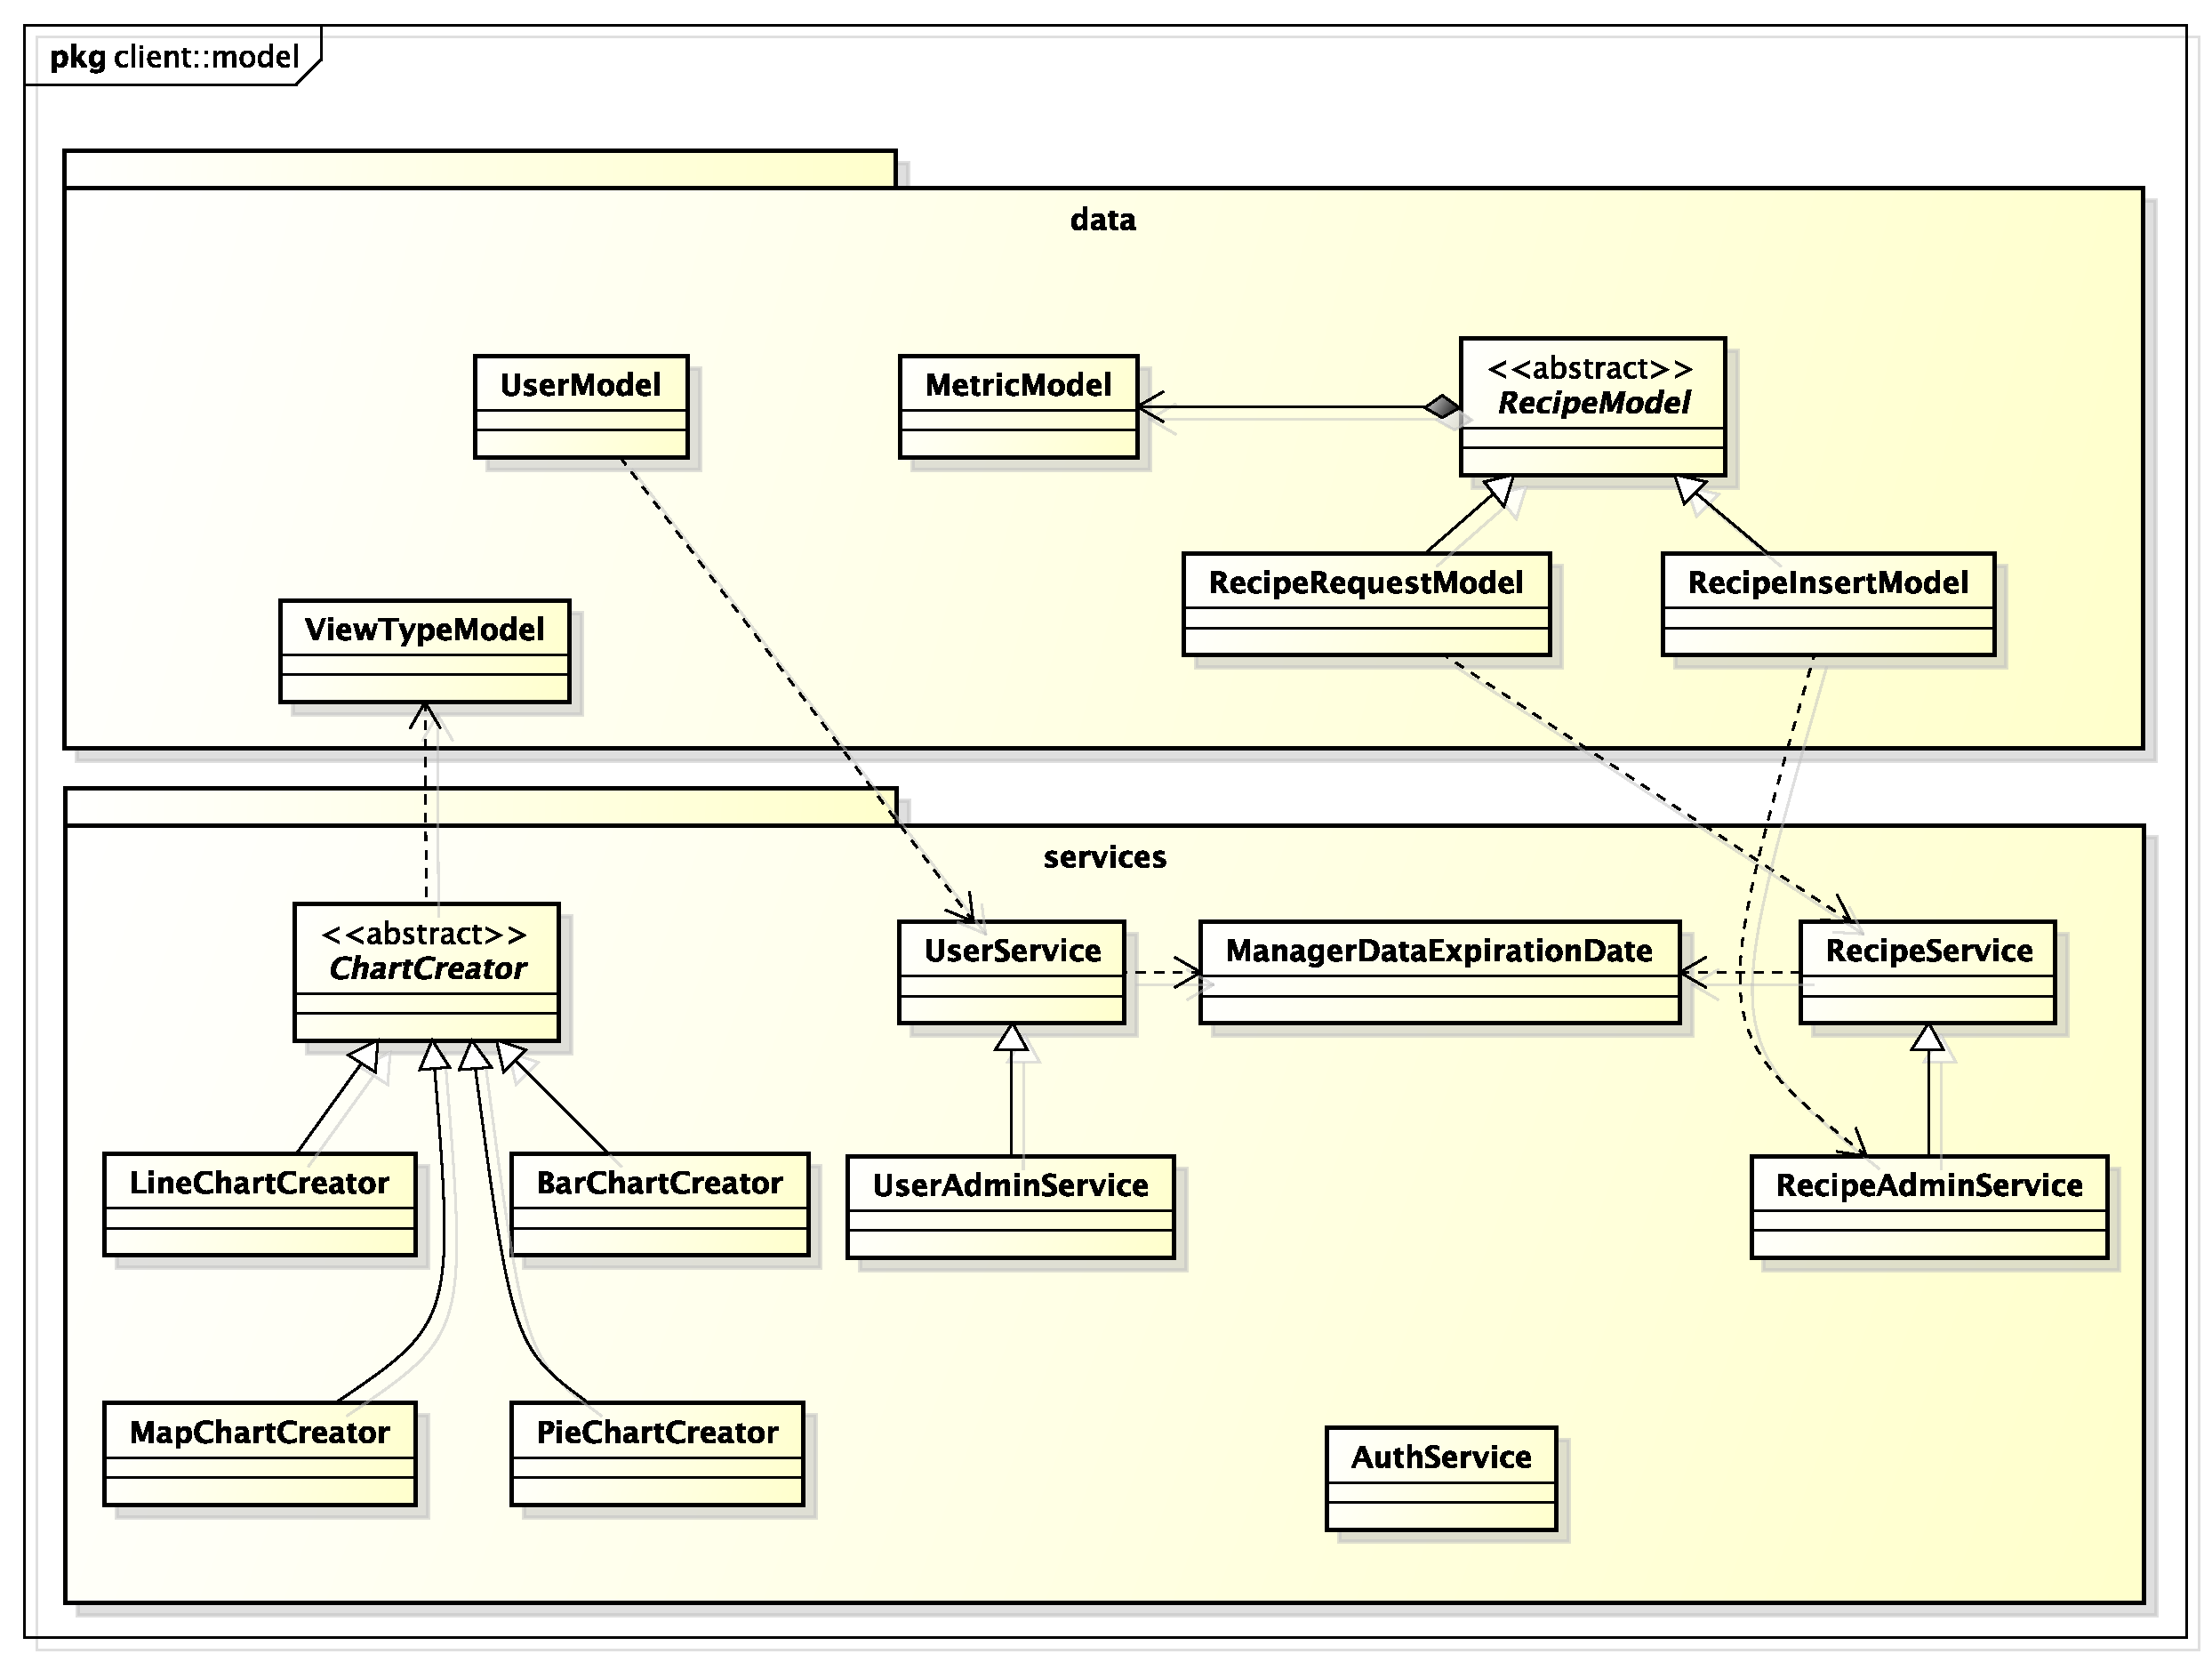
\includegraphics[scale=0.45]{./images/client_model.pdf}}
	\caption{Package - client::model}
\end{figure}

\begin{itemize}
	\item \textbf{Descrizione}: è il package che contiene sia le classi dei modelli di dati utilizzati dal client sia i servizi che mettono in comunicazione esso con il server attraverso i diversi servizi REST;
	\item \textbf{Padre}: client;
	\item \textbf{Package contenuti}:
		\begin{itemize}
			\item client::model::data
			\item client::model::services
		\end{itemize}
	\item \textbf{Interazione con altri componenti}:
		\begin{itemize}
			\item client::controller
		\end{itemize}
\end{itemize}
% subsubsection bdsm_app_client_model (end)

% PACKAGE MODEL::DATA
% =================================================================================================
% File:			client_tier/model/data.tex
% Description:	Defiinisce la sezione relativa al front-end dell'applicazione
% Created:		2015-04-10
% Author:		Tesser Paolo
% Email:		tesser.paolo@mashup-unipd.it
% =================================================================================================
% Modification History:
% Version		Modifier Date		Change											Author
% 0.0.1 		2015-04-10 			creato scheletro								Tesser Paolo
% =================================================================================================
% 0.0.2			2015-04-11			scheletro classi contenuti nei package			Tesser Paolo
% =================================================================================================
%

% CONTENUTO DEL CAPITOLO
%

\subsubsection{bdsm\_app::client::model::data} % (fold)
\label{ssub:bdsm_app_client_model_data}
\begin{figure}[htbp]
	\centering
	\centerline{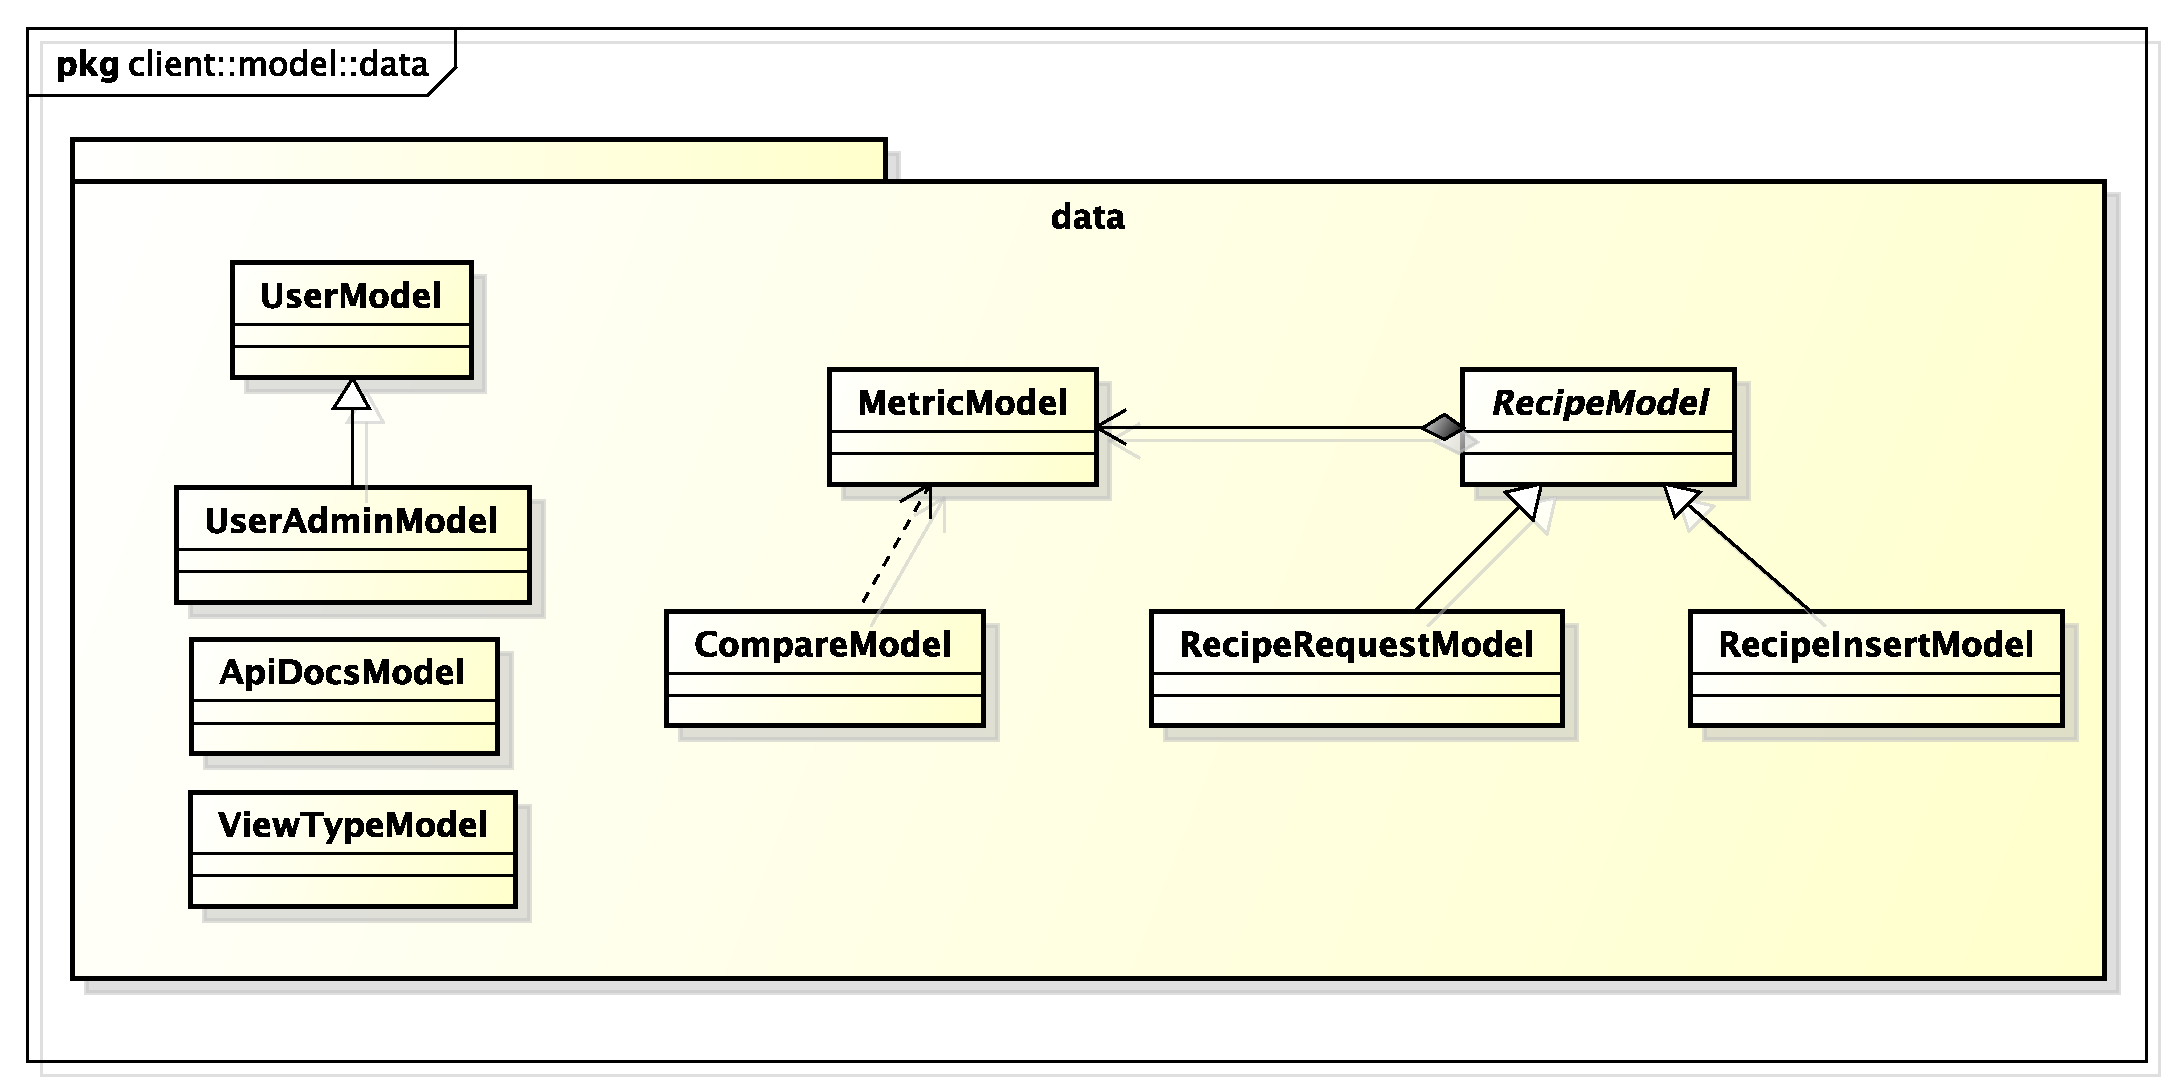
\includegraphics[scale=0.5]{./images/client_model_data.pdf}}
	\caption{Package - client::model::data}
\end{figure}

\begin{itemize}
	\item \textbf{Descrizione}: è il package c;
	\item \textbf{Padre}: client::model
	\item \textbf{Interazione con altri componenti}:
		\begin{itemize}
			\item client::model::services
			\item client::controller
		\end{itemize}

	\paragraph{Classi} % (fold)

		\subparagraph{client::model::data::ViewTypeModel} % (fold)
		\label{subp:client_model_data_viewtypemodel}
			\begin{itemize}
				\item \textbf{Descrizione}: [TO DO];
				\item \textbf{Utilizzo}: [TO DO];
				\item \textbf{Classi ereditate}: [TO DO];
				\item \textbf{Relazioni con altre classi}: [TO DO].
			\end{itemize}
		% subparagraph client_model_data_viewtypedata (end)


		\subparagraph{client::model::data::UserModel} % (fold)
		\label{subp:client_model_data_user}
			\begin{itemize}
				\item \textbf{Descrizione}: [TO DO];
				\item \textbf{Utilizzo}: [TO DO];
				\item \textbf{Classi ereditate}: [TO DO];
				\item \textbf{Relazioni con altre classi}: [TO DO].
			\end{itemize}
		% subparagraph client_model_data_user (end)

		\subparagraph{client::model::data::RecipeModel} % (fold)
		\label{subp:client_model_data_recipe}
			\begin{itemize}
				\item \textbf{Descrizione}: [TO DO];
				\item \textbf{Utilizzo}: [TO DO];
				\item \textbf{Classi ereditate}: [TO DO];
				\item \textbf{Relazioni con altre classi}: [TO DO].
			\end{itemize}
		% subparagraph client_model_data_recipe (end)

		\subparagraph{client::model::data::RecipeRequestModel} % (fold)
		\label{subp:client_model_data_reciperequestmodel}
			\begin{itemize}
				\item \textbf{Descrizione}: [TO DO];
				\item \textbf{Utilizzo}: [TO DO];
				\item \textbf{Classi ereditate}: [TO DO];
				\item \textbf{Relazioni con altre classi}: [TO DO].
			\end{itemize}
		% subparagraph client_model_data_reciperequestmodel (end)

		\subparagraph{client::model::data::RecipeInsertModel} % (fold)
		\label{subp:client_model_data_recipeinsertmodel}
			\begin{itemize}
				\item \textbf{Descrizione}: [TO DO];
				\item \textbf{Utilizzo}: [TO DO];
				\item \textbf{Classi ereditate}: [TO DO];
				\item \textbf{Relazioni con altre classi}: [TO DO].
			\end{itemize}
		% subparagraph client_model_data_recipeinsertmodel (end)

		\subparagraph{client::model::data::MetricModel} % (fold)
		\label{subp:client_model_data_metricmodel}
			\begin{itemize}
				\item \textbf{Descrizione}: [TO DO];
				\item \textbf{Utilizzo}: [TO DO];
				\item \textbf{Classi ereditate}: [TO DO];
				\item \textbf{Relazioni con altre classi}: [TO DO].
			\end{itemize}
		% subparagraph client_model_data_metricmodel (end)


\end{itemize}
% subsubsection bdsm_app_client_model_data (end) % \clearpage \newpage
% END PACKAGE MODEL::DATA

% PACKAGE MODEL::SERVICES
% =================================================================================================
% File:			client_tier/model/services.tex
% Description:	Defiinisce la sezione relativa al front-end dell'applicazione
% Created:		2015-04-10
% Author:		Tesser Paolo
% Email:		tesser.paolo@mashup-unipd.it
% =================================================================================================
% Modification History:
% Version		Modifier Date		Change											Author
% 0.0.1 		2015-04-10 			creato scheletro								Tesser Paolo
% =================================================================================================
%
%

% CONTENUTO DEL CAPITOLO
%

\subsubsection{bdsm\_app::client::model::services} % (fold)
\label{ssub:bdsm_app_client_model_services}
\begin{figure}[htbp]
	\centering
	\centerline{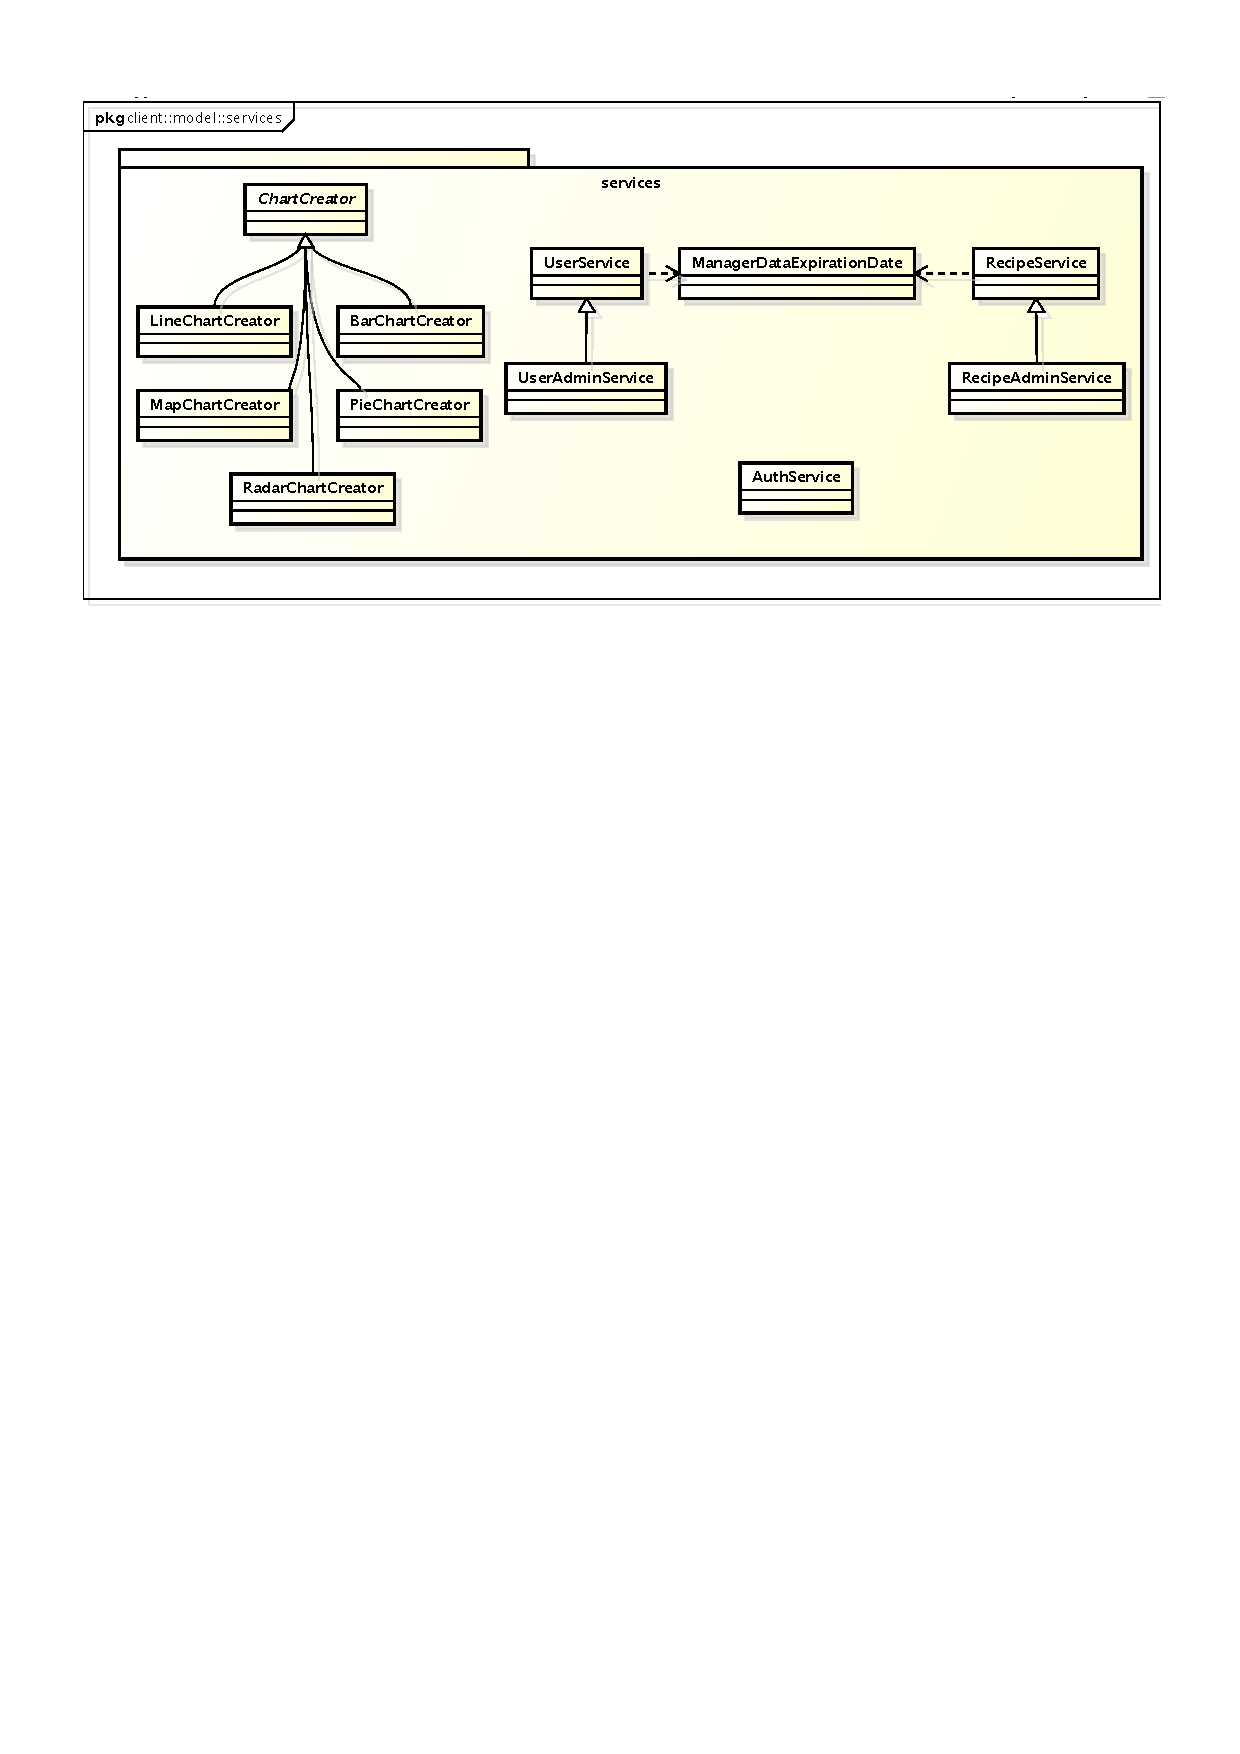
\includegraphics[scale=1.00]{./images/client_model_services.pdf}}
	\caption{Package - client::model}
\end{figure}

\begin{itemize}
	\item \textbf{Descrizione}: È il package che contiene le classi che sviluppano il core business dell'applicazione: in particolare gestiscono il recupero dei dati, siano essi salvati in locale o da recuperare chiamando il server, la crezione dei grafici e l'autenticazione.
	Tutte le classi contenute in questo package implementano il pattern \emph{Singleton};
	\item \textbf{Padre}: client::model
	\item \textbf{Interazione con altri componenti}:
		\begin{itemize}
			\item client::model::data
			\item client::controller
		\end{itemize}
	
	\paragraph{Classi} % (fold)

		\subparagraph{client::model::services::AuthService} % (fold)
		\label{subp:client_model_services_authservice}
			\begin{itemize}
				\item \textbf{Descrizione}: È la classe che implementa un \emph{Adapter} per gestire le chiamate al modulo esterno usato per gestire l'autenticazione;
				\item \textbf{Utilizzo}: I metodi di questa classe saranno invocati quando un utente effettua la registrazione al servizio o effettua un login/logout;
				\item \textbf{Relazioni con altre classi}: 					
					\begin{itemize}
						\item client::controller::public::LoginCtrl
						\item client::controller::public::RegisterCtrl
						\item client::controller::user::LogoutCtrl
					\end{itemize}
			\end{itemize}
		
		\subparagraph{client::model::services::RecipeService} % (fold)
		\label{subp:client_model_services_recipeservice}
			\begin{itemize}
				\item \textbf{Descrizione}: È la classe che racchiude i metodi per reperire i dati relativi alle Recipe, siano essi salvati in locale o da recuperare dal server, inoltre gestisce l'invio di richieste di Recipe al server;
				\item \textbf{Utilizzo}: I suoi metodi vengono invocati ogni volta che sia necessario avere dei dati relativi a una o più Recipe per un utente non amministratore, o se un utente non amministratore desidera inviare una richiesta di Recipe;
				\item \textbf{Relazioni con altre classi}: 					
					\begin{itemize}
						\item client::model::data::RecipeRequestModel
						\item client::model::services::ManagerDataExpirationDate
						\item client::controller::user::RecipeCtrl
						\item client::controller::user::MetricsCtrl
						\item client::controller::user::ChartsCtrl						
						\item client::controller::user::CompareCtrl
					\end{itemize}
			\end{itemize}
		% subparagraph client_model_services_recipeservice (end)

		\subparagraph{client::model::services::RecipeAdminService} % (fold)
		\label{subp:client_model_services_recipeadminservice}
			\begin{itemize}
				\item \textbf{Descrizione}: È la classe che oltre a gestire ciò che è gestito dalla classe padre si occupa dell'inserimento di nuove recipe nel server e dell'eliminazione di Recipe già presenti;
				\item \textbf{Utilizzo}: I suoi metodi vengono invocati quando un utente amministratore desidera agire su dati di Recipe da pagine non accessibili a un utente non amministratore;
				\item \textbf{Classi ereditate}:					
					\begin{itemize}
						\item client::model::services::RecipeService
					\end{itemize}
				\item \textbf{Relazioni con altre classi}:
					\begin{itemize}
						\item client::model::data::RecipeInsertModel
						\item client::model::services::ManagerDataExpirationDate
						\item client::controller::admin::RecipeConfigCtrl
						\item client::controller::admin::InsertRecipeCtrl
					\end{itemize}
			\end{itemize}
		% subparagraph client_model_services_recipeadminservice (end)


		\subparagraph{client::model::services::UserService} % (fold)
		\label{subp:client_model_services_userservice}
			\begin{itemize}
				\item \textbf{Descrizione}: È la classe che gestisce il recupero e la modifica di dati utente relativi a sé stessi;
				\item \textbf{Utilizzo}: I suoi metodi vengono invocati quando un utente accede alla pagina dei propri dati personali;
				\item \textbf{Relazioni con altre classi}:
					\begin{itemize}
						\item client::model::data::UserModel
						\item client::model::services::ManagerDataExpirationDate
						\item client::controller::user::SettingsCtrl
					\end{itemize}
			\end{itemize}
		% subparagraph client_model_services_userservice (end)

		\subparagraph{client::model::services::UserAdminService} % (fold)
		\label{subp:client_model_services_useradminservice}
			\begin{itemize}
				\item \textbf{Descrizione}: È la classe che oltre a gestire ciò che è gestito dalla sua classe padre si occupa del recupero e della modifica di dati di utenti, inclusa l'eliminazione di un utente e il cambiare i suoi permessi;
				\item \textbf{Utilizzo}: I suoi metodi vengono invocati quando un utente amministratore agisce su dati relativi ad utenti da una pagina non accessibile agli utenti non amministratori;
				\item \textbf{Classi ereditate}:					
					\begin{itemize}
						\item client::model::services::UserService
					\end{itemize}
				\item \textbf{Relazioni con altre classi}:
					\begin{itemize}
						\item client::model::data::UserModel
						\item client::model::services::ManagerDataExpirationDate
						\item client::controller::user::UserConfigCtrl
					\end{itemize}
				\end{itemize}
		% subparagraph client_model_services_useradminservice (end)

		\subparagraph{client::model::services::ChartCreator} % (fold)
		\label{subp:chartcreator}
			\begin{itemize}
				\item \textbf{Descrizione}: È una classe astratta che descrive il codice comune delle classi che generano un grafico, secondo il pattern \emph{template method};
				\item \textbf{Utilizzo}: I suoi metodi vengono invocati dalle classi figlie nella creazione di grafici;
				\item \textbf{Relazioni con altre classi}:
					\begin{itemize}
						\item client::model::data::ViewTypeModel
						\item client::model::services::LineChartCreator
						\item client::model::services::BarChartCreator
						\item client::model::services::MapChartCreator
						\item client::model::services::PieChartCreator
						\item client::model::services::RadarChartCreator
						\item client::controller::user::ChartsCtrl
						\item client::controller::user::CompareCtrl
					\end{itemize}
			\end{itemize}
		% subparagraph chartcreator (end)

		\subparagraph{client::model::services::LineChartCreator} % (fold)
		\label{subp:linechartcreator}
			\begin{itemize}
				\item \textbf{Descrizione}: La classe contiene i metodi per la creazione di un Line Chart;
				\item \textbf{Utilizzo}: I suoi metodi vengono invocati quando si vuole creare un Line Chart;
				\item \textbf{Classi ereditate}:					
					\begin{itemize}
						\item client::model::services::ChartCreator
					\end{itemize}
				\item \textbf{Relazioni con altre classi}:					
					\begin{itemize}
						\item client::controller::user::ChartsCtrl
						\item client::controller::user::CompareCtrl
					\end{itemize}
			\end{itemize}
		% subparagraph linechartcreator (end)


		\subparagraph{client::model::services::BarChartCreator} % (fold)
		\label{subp:barchartcreator}
			\begin{itemize}
				\item \textbf{Descrizione}: La classe contiene i metodi per la creazione di un Bar Chart;
				\item \textbf{Utilizzo}: I suoi metodi vengono invocati quando si vuole creare un Bar Chart;
				\item \textbf{Classi ereditate}:					
					\begin{itemize}
						\item client::model::services::ChartCreator
					\end{itemize}
				\item \textbf{Relazioni con altre classi}:					
					\begin{itemize}
						\item client::controller::user::ChartsCtrl
						\item client::controller::user::CompareCtrl
					\end{itemize}
			\end{itemize}
		% subparagraph barchartcreator (end)

		\subparagraph{client::model::services::PieChartCreator} % (fold)
		\label{subp:piechartcreator}
			\begin{itemize}
				\item \textbf{Descrizione}: La classe contiene i metodi per la creazione di un Pie Chart;
				\item \textbf{Utilizzo}: I suoi metodi vengono invocati quando si vuole creare un Pie Chart;
				\item \textbf{Classi ereditate}:					
					\begin{itemize}
						\item client::model::services::ChartCreator
					\end{itemize}
				\item \textbf{Relazioni con altre classi}:					
					\begin{itemize}
						\item client::controller::user::ChartsCtrl
						\item client::controller::user::CompareCtrl
					\end{itemize}
			\end{itemize}
		% subparagraph piechartcreator (end)

		\subparagraph{client::model::services::MapChartCreator} % (fold)
		\label{subp:mapchartcreator}
			\begin{itemize}
				\item \textbf{Descrizione}: La classe contiene i metodi per la creazione di un Map Chart;
				\item \textbf{Utilizzo}: I suoi metodi vengono invocati quando si vuole creare un Map Chart;
				\item \textbf{Classi ereditate}:					
					\begin{itemize}
						\item client::model::services::ChartCreator
					\end{itemize}
				\item \textbf{Relazioni con altre classi}:					
					\begin{itemize}
						\item client::controller::user::ChartsCtrl
						\item client::controller::user::CompareCtrl
					\end{itemize}
			\end{itemize}
		% subparagraph mapchartcreator (end)

		\subparagraph{client::model::services::RadarChartCreator} % (fold)
		\label{subp:radarchartcreator}
			\begin{itemize}
				\item \textbf{Descrizione}: La classe contiene i metodi per la creazione di un Radar Chart;
				\item \textbf{Utilizzo}: I suoi metodi vengono invocati quando si vuole creare un Radar Chart;
				\item \textbf{Classi ereditate}:					
					\begin{itemize}
						\item client::model::services::ChartCreator
					\end{itemize}
				\item \textbf{Relazioni con altre classi}:					
					\begin{itemize}
						\item client::controller::user::ChartsCtrl
						\item client::controller::user::CompareCtrl
					\end{itemize}
			\end{itemize}
		% subparagraph radarchartcreator (end)

		\subparagraph{client::model::services::ManagerDataExpirationDate} % (fold)
		\label{subp:radarchartcreator}
			\begin{itemize}
				\item \textbf{Descrizione}: Questa classe controlla se i dati che vengono richiesti sono già presenti in locale o se devono essere richiesti al server: in particolare li richiede al server solo se questi sono assenti o se sono l'ultima volta che sono stati chiesti al server è passata da troppo tempo;
				\item \textbf{Utilizzo}: I suoi metodi vengono invocati dalle classi che desiderano fare richieste al server;
				\item \textbf{Relazioni con altre classi}:					
					\begin{itemize}
						\item client::model::services::RecipeService
						\item client::model::services::RecipeAdminService
						\item client::model::services::UserService
						\item client::model::services::UserAdminService
					\end{itemize}
			\end{itemize}
		% subparagraph managerdataexpirationdate (end)


\end{itemize}
% subsubsection bdsm_app_client_model_services (end)
% END PACKAGE MODEL::SERVICES \clearpage \newpage
	% END PACKAGE MODEL

	% PACKAGE DELLA VIEW
	% =================================================================================================
% File:			client_tier/view.tex
% Description:	Defiinisce la sezione relativa al front-end dell'applicazione
% Created:		2015-04-07
% Author:		Tesser Paolo
% Email:		tesser.paolo@mashup-unipd.it
% =================================================================================================
% Modification History:
% Version		Modifier Date		Change											Author
% 0.0.1 		2015-04-07 			creato scheletro								Tesser Paolo
% =================================================================================================
% 0.0.2			2015-04-07			descrizione delle classi						Carnovalini Filippo
% =================================================================================================
% 0.0.3			2015-04-08			aggiunte classi sulle relazioni					Tesser Paolo
% =================================================================================================
%

% CONTENUTO DEL CAPITOLO

\subsubsection{bdsm\_app::client::view} % (fold)
\label{ssub:bdsm_app_client_view}
In questa sezione e in tutte quelle inerenti al package \textbf{view}, il termine classe e pagina HTML, saranno sinonimi.
\begin{figure}[htbp]
	\centering
	\centerline{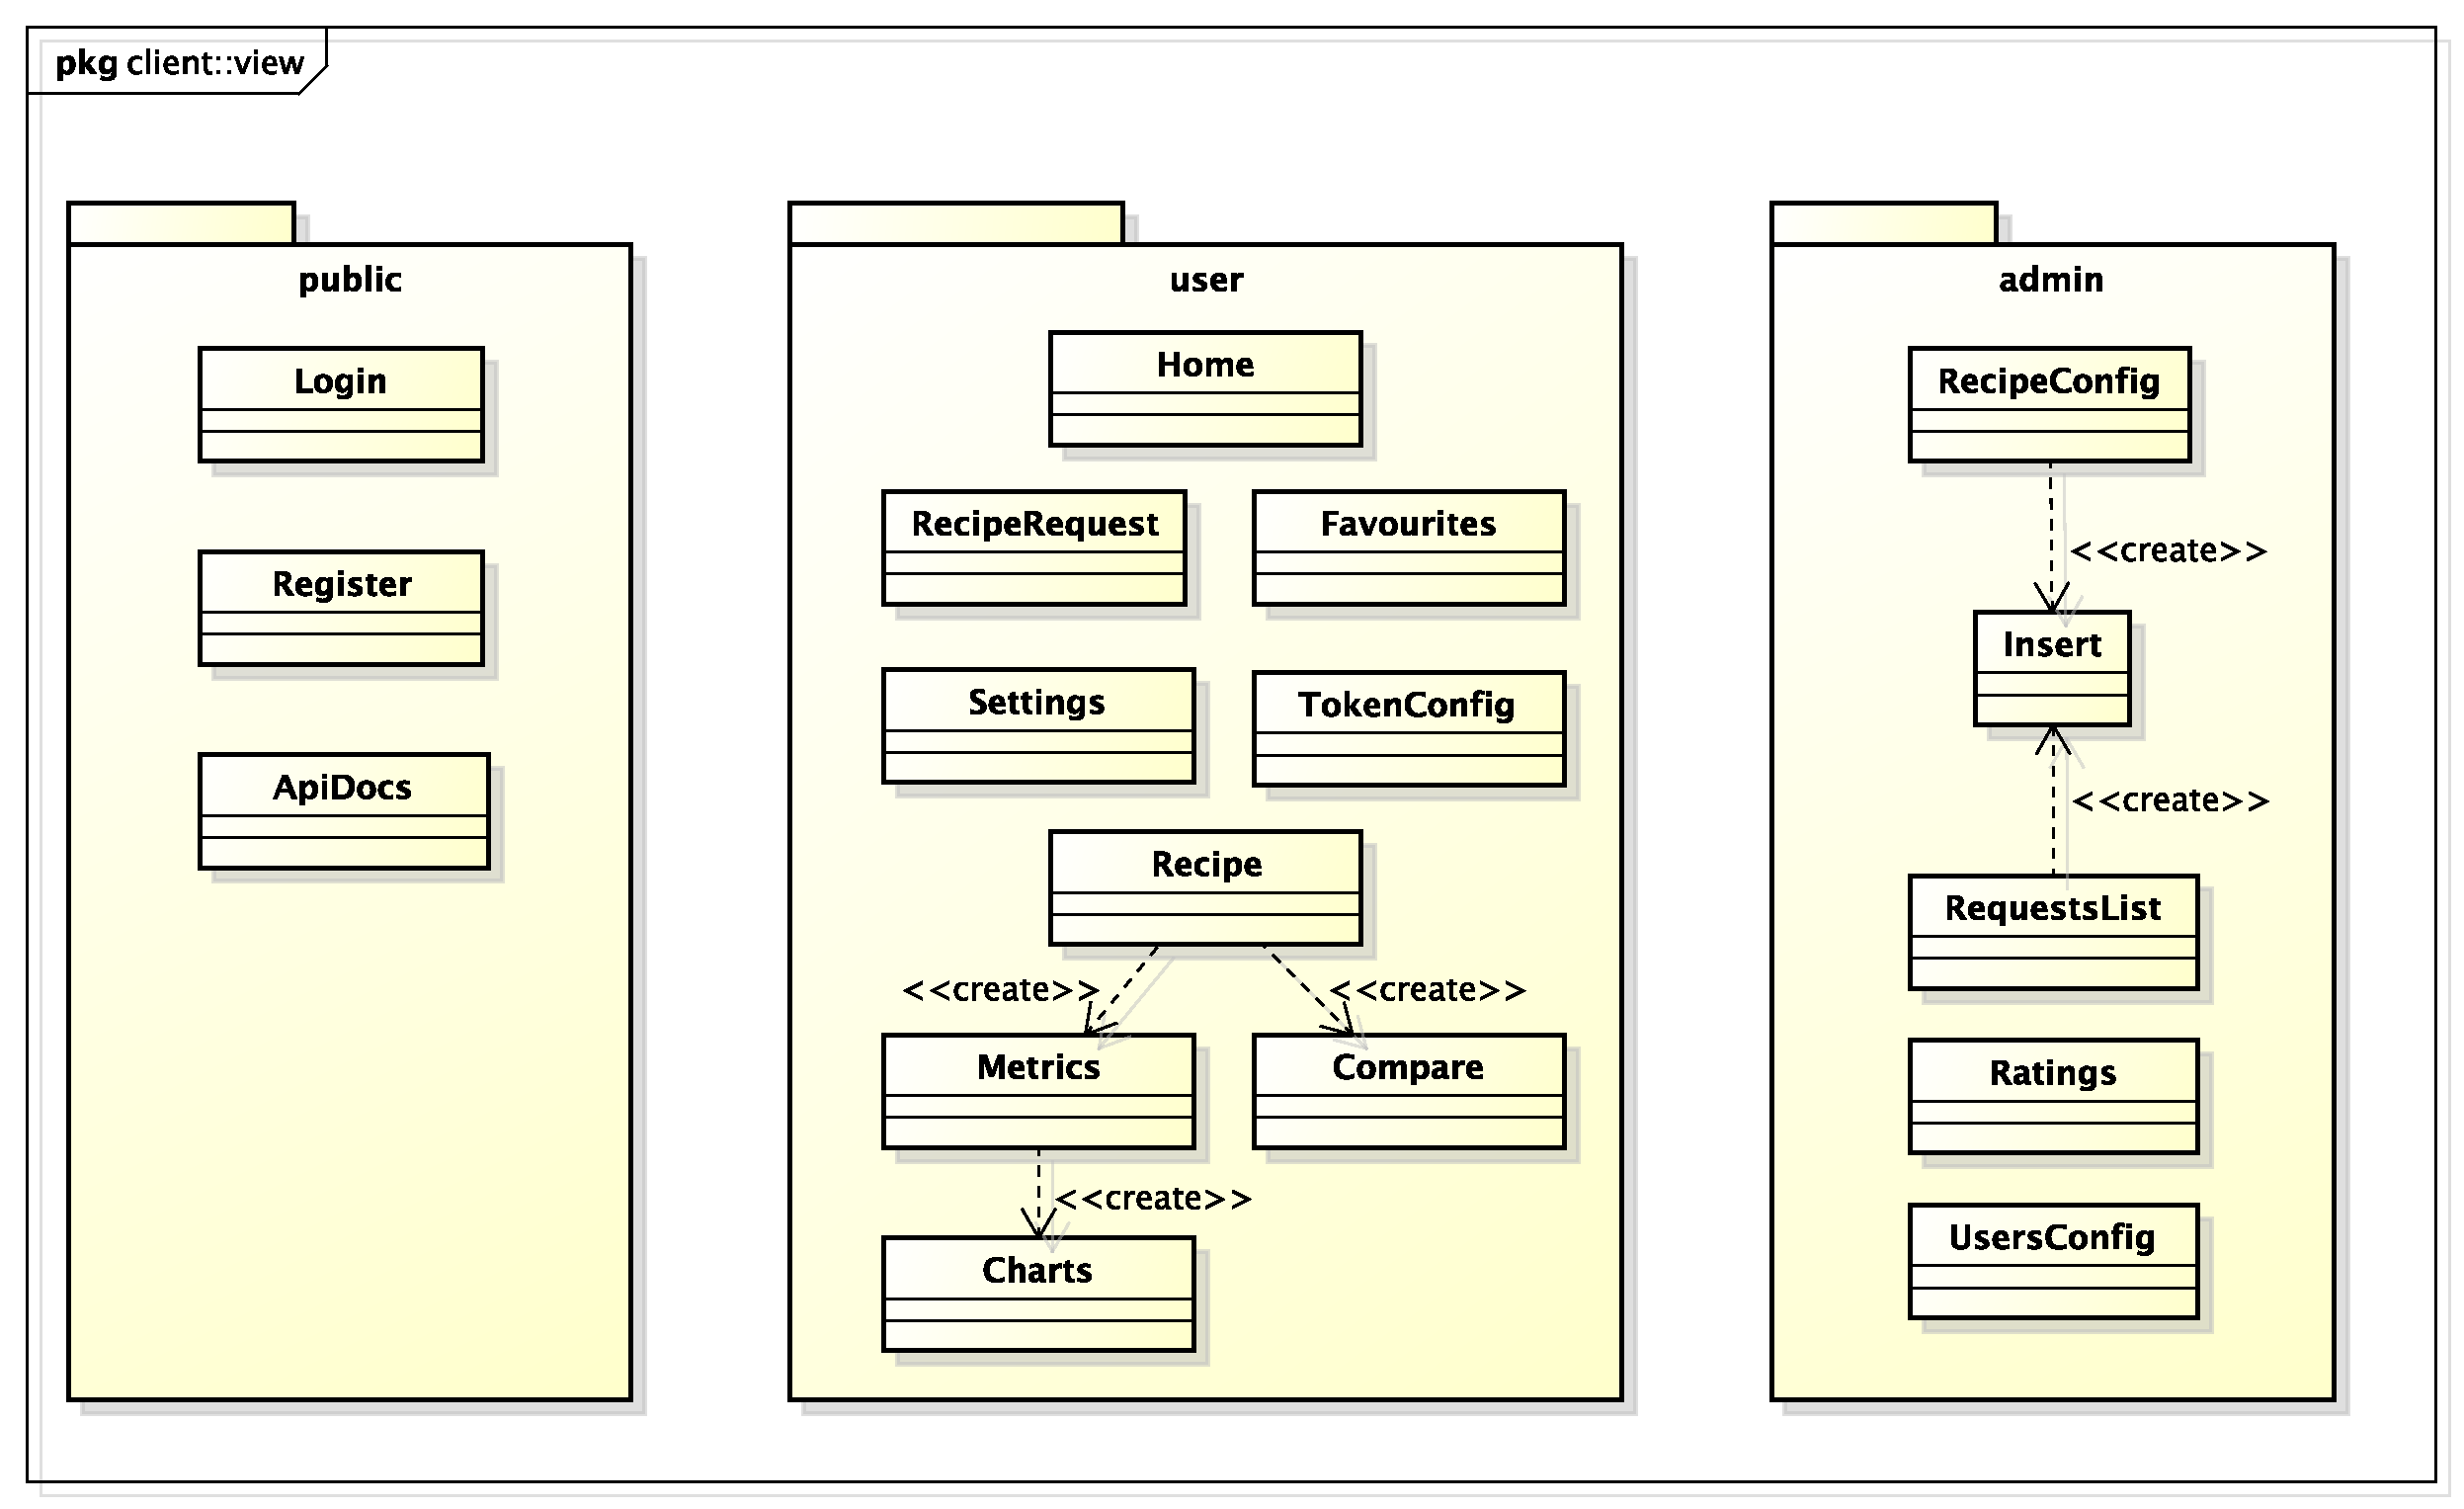
\includegraphics[scale=0.5]{./images/client_view.pdf}}
	\caption{Package - client::view}
\end{figure}

\begin{itemize}
	\item \textbf{Descrizione}: è il package che contiene tutte le classi che costituiscono la view del client. Ogni classe è equivalenti a un template di pagina HTML che sarà presentato all'utente, quando richiesto, tramite un sistema di routing. \newline
	All'interno di esso sono presenti altri componenti che separano le pagine HTML offerte, a seconda dei permessi che possiede un utente;
	\item \textbf{Padre}: client
	\item \textbf{Package contenuti}:
		\begin{itemize}
			\item client::view::public
			\item client::view::user
			\item client::view::admin
		\end{itemize}
	\item \textbf{Interazione con altri componenti}:
		\begin{itemize}
			\item client::controller
		\end{itemize}
\end{itemize}
% subsubsection bdsm_app_client_view (end)

\pagebreak

\subsubsection{bdsm\_app::client::view::public} % (fold)
\label{ssub:bdsm_app_client_view_public}
\begin{figure}[htbp]
	\centering
	\centerline{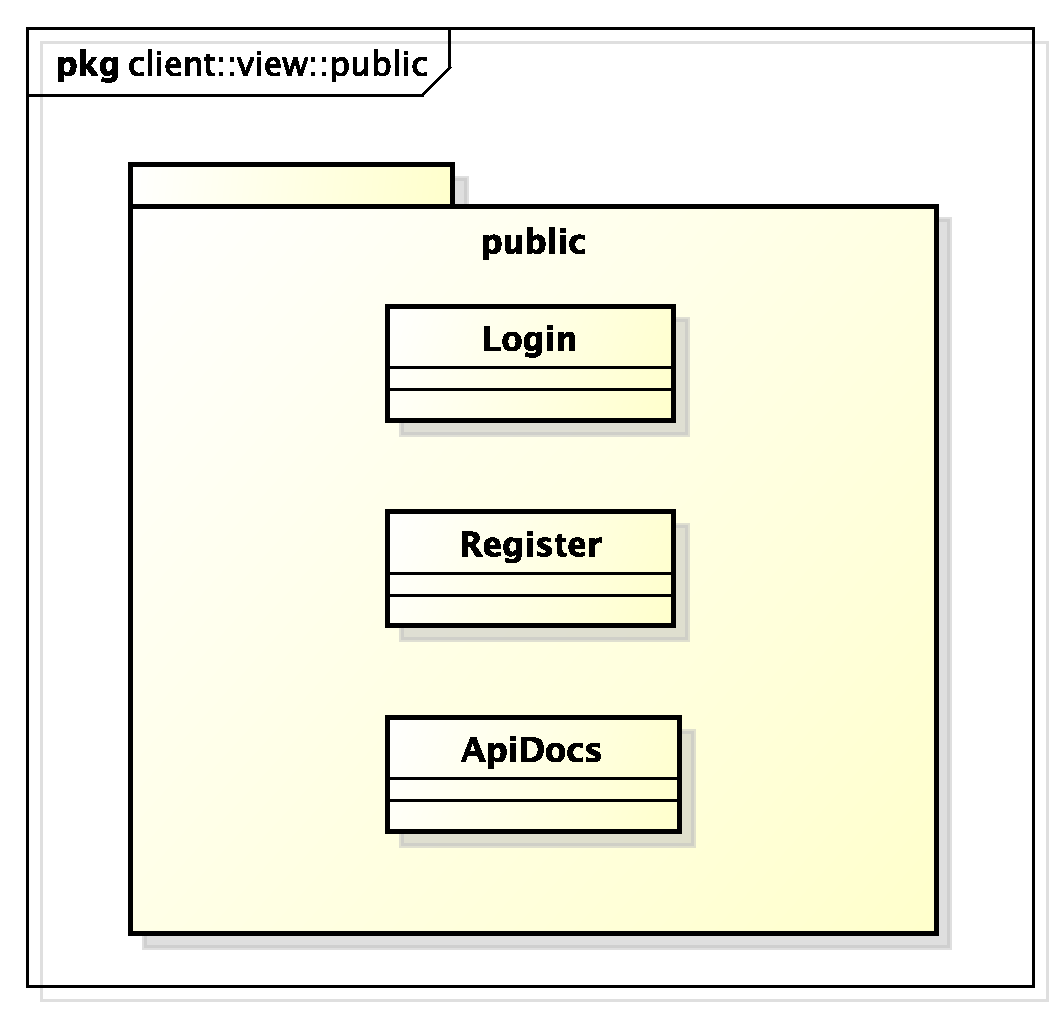
\includegraphics[scale=0.6]{./images/client_view_public.pdf}}
	\caption{Package - client::view::public}
\end{figure}

\begin{itemize}
	\item \textbf{Descrizione}: è il package che contiene tutte le pagine HTML che possono essere offerte quando l'utente deve ancora effettuare l'accesso al sistema;
	\item \textbf{Padre}: client::view
	\item \textbf{Interazione con altri componenti}: 
		\begin{itemize}
			\item client::controller::public
		\end{itemize}
\end{itemize}

	\paragraph{Classi} % (fold)
		\subparagraph{bdsm\_app::client::view::public::Login} % (fold)
		\label{subp:bdsm_app_client_view_public_login}
			\begin{itemize}
				\item \textbf{Descrizione}: La classe rappresenta un template HTML per la visualizzazione dell'interfaccia di autenticazione;
				\item \textbf{Utilizzo}: Viene utilizzata per generare la pagina HTML di autenticazione;
				\item \textbf{Relazioni con altre classi}:
					\begin{itemize}
						\item client::controller::public::PublicRoute
						\item client::controller::public::LoginCtrl
					\end{itemize}
			\end{itemize}
		% subparagraph bdsm_app_client_view_public_login (end)

		\subparagraph{bdsm\_app::client::view::public::About} % (fold)
		\label{subp:bdsm_app_client_view_public_about}
			\begin{itemize}
				\item \textbf{Descrizione}: La classe rappresenta un template HTML per la visualizzazione della pagina di informazioni sull'applicazione;
				\item \textbf{Utilizzo}: Viene usata per generare la pagina HTML di About;
				\item \textbf{Relazioni con altre classi}:
					\begin{itemize}
						\item client::controller::public::PublicRoute
					\end{itemize}
			\end{itemize}
		% subparagraph bdsm_app_client_view_public_about (end)

		\subparagraph{bdsm\_app::client::view::public::Register} % (fold)
		\label{subp:bdsm_app_client_view_public_register}
			\begin{itemize}
				\item \textbf{Descrizione}: La classe rappresenta un template HTML per la visualizzazione dell'interfaccia di registrazione al servizio;
				\item \textbf{Utilizzo}: Viene utilizzata per generare la pagina HTML di registrazione;
				\item \textbf{Relazioni con altre classi}:
					\begin{itemize}
						\item client::controller::public::PublicRoute
						\item client::controller::public::RegisterCtrl
					\end{itemize}
			\end{itemize}
		% subparagraph bdsm_app_client_view_public_register (end)

		\subparagraph{bdsm\_app::client::view::public::ApiDocs} % (fold)
		\label{subp:bdsm_app_client_view_public_apidocs}
			\begin{itemize}
				\item \textbf{Descrizione}: La classe rappresenta un template HTML per la visualizzazione della pagina contenente la documentazione dei servizi REST offerti;
				\item \textbf{Utilizzo}: Viene utilizzata per generare la pagina HTML contenente la documentazione dei servizi offerti;
				\item \textbf{Relazioni con altre classi}: 		
					\begin{itemize}
						\item client::controller::public::PublicRoute
						\item client::controller::public::ApiDocsCtrl
					\end{itemize}
			\end{itemize}
		% subparagraph bdsm_app_client_view_public_apidocs (end)

% subsubsection bdsm_app_client_view_public (end)


\subsubsection{bdsm\_app::client::view::user} % (fold)
\label{ssub:bdsm_app_client_view_user}
\begin{figure}[htbp]
	\centering
	\centerline{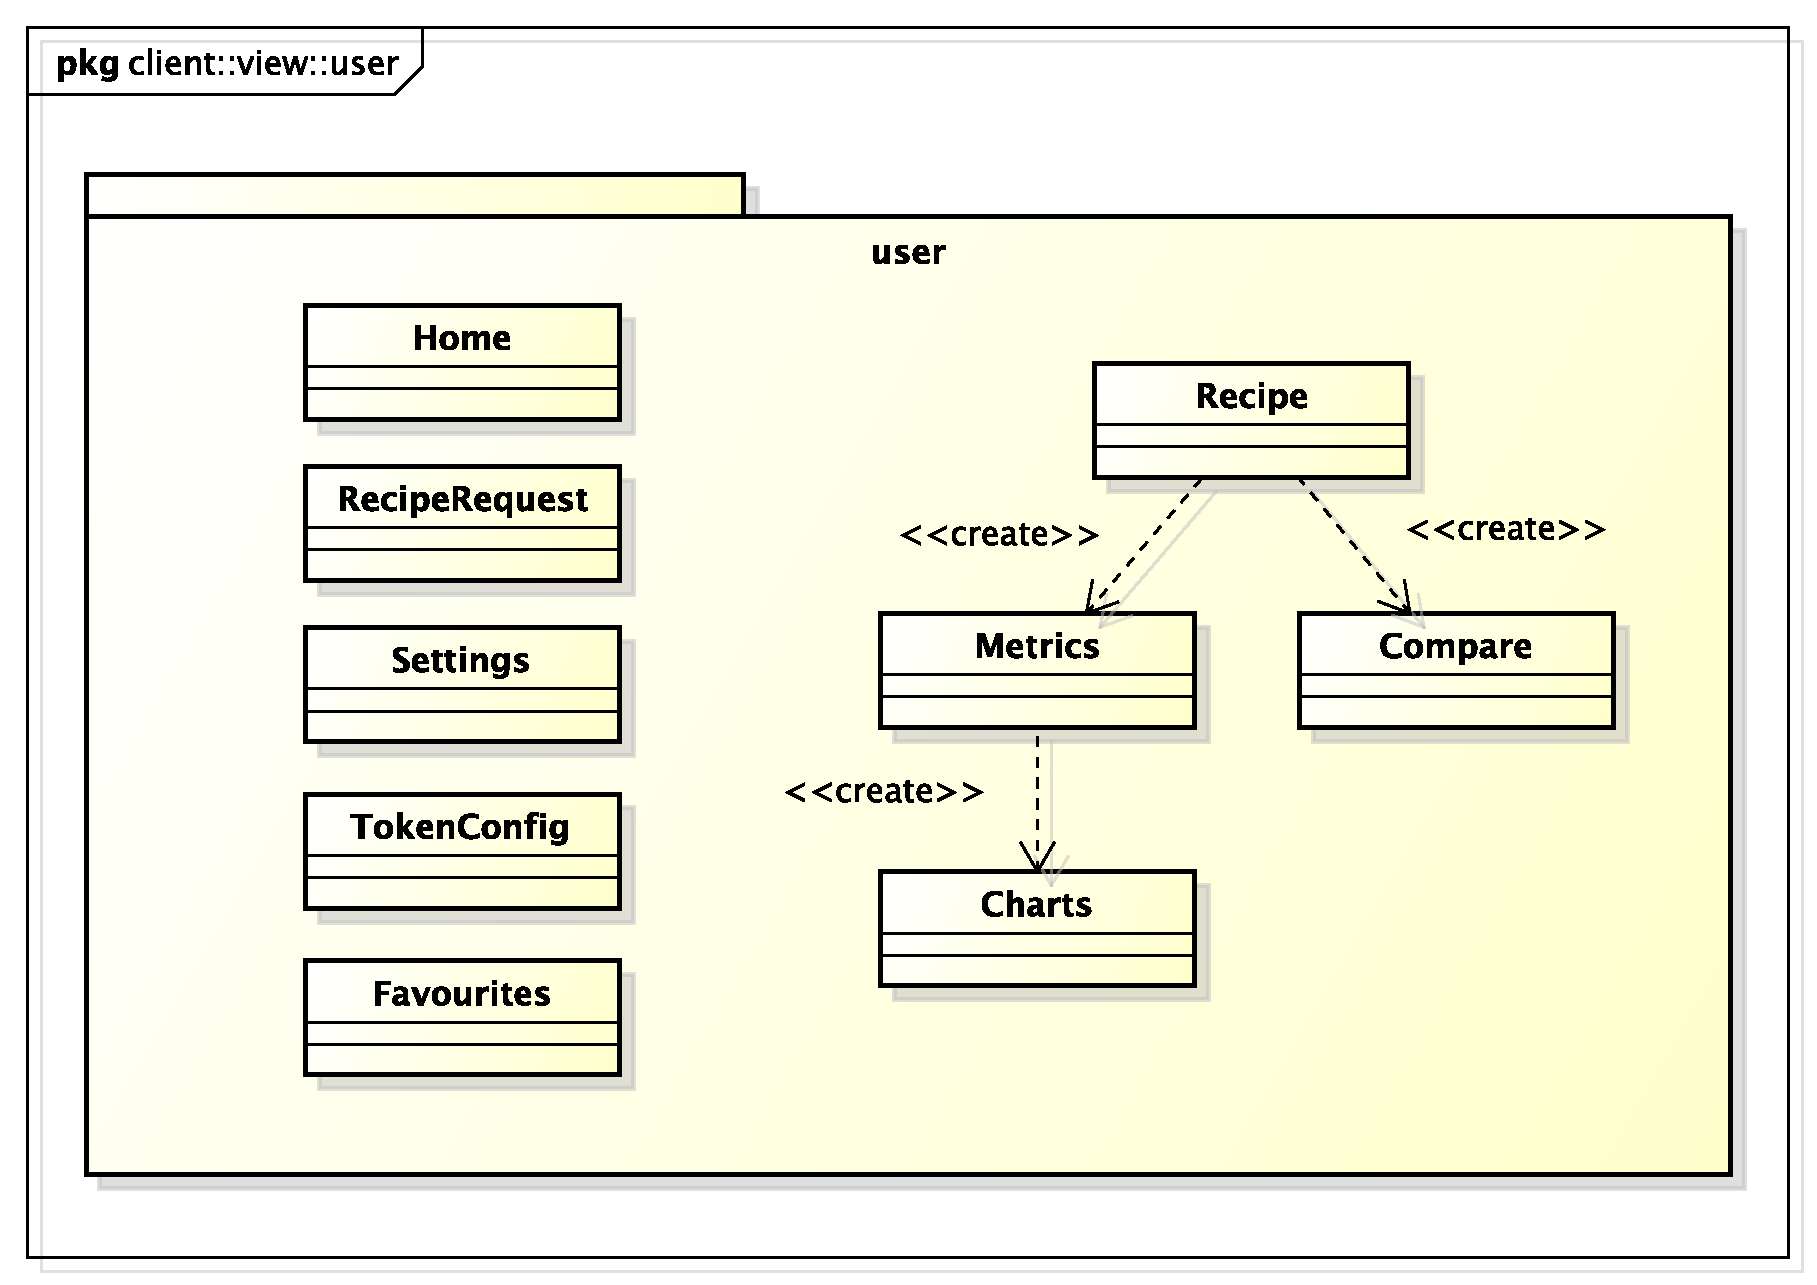
\includegraphics[scale=0.8]{./images/client_view_user.pdf}}
	\caption{Package - client::view::user}
\end{figure}

\begin{itemize}
	\item \textbf{Descrizione}: è il package che contiene tutte le pagine HTML che ha a disposizione l'utente che ha effettuato l'accesso al sistema, sia che sia un utente normale sia che sia un amministratore. \newline
	Per semplicità e chiarezza non è stato evidenziato nel grafico il fatto che ogni classe di questo package possiede un'istanza di MenuMain e di MenuSecond.
	\item \textbf{Padre}: client::view
	\item \textbf{Interazione con altri componenti}:
		\begin{itemize}
			\item client::controller::user
		\end{itemize}
\end{itemize}

	\paragraph{Classi} % (fold)
		\subparagraph{bdsm\_app::client::view::user::Home} % (fold)
		\label{subp:bdsm_app_client_view_user_home}
			\begin{itemize}
				\item \textbf{Descrizione}: La classe rappresenta un template HTML per la visualizzazione dell'interfaccia della home dell'applicazione;
				\item \textbf{Utilizzo}: Viene utilizzata per generare la pagina HTML della home;
				\item \textbf{Relazioni con altre classi}:
					\begin{itemize}
						\item client::view::user::MenuMain
						\item client::view::user::MenuSecond
						\item client::controller::public::HomeRoute
						\item client::controller::user::HomeCtrl
					\end{itemize}
			\end{itemize}
		% subparagraph bdsm_app_client_view_user_home (end)

		\subparagraph{bdsm\_app::client::view::user::Recipe} % (fold)
		\label{subp:bdsm_app_client_view_user_recipe}
			\begin{itemize}
				\item \textbf{Descrizione}: La classe rappresenta un template HTML per la visualizzazione della pagina di visione delle recipe a disposizione;
				\item \textbf{Utilizzo}: Viene usata per generare la pagina HTML di visione delle recipe;
				\item \textbf{Relazioni con altre classi}:
					\begin{itemize}
						\item client::view::user::MenuMain
						\item client::view::user::MenuSecond
						\item client::view::user::Metrics
						\item client::view::user::Compare
						\item client::controller::user::RecipeRoute
						\item client::controller::user::RecipeCtrl
					\end{itemize}
			\end{itemize}
		% subparagraph bdsm_app_client_view_user_recipe (end)

		\subparagraph{bdsm\_app::client::view::user::Metrics} % (fold)
		\label{subp:bdsm_app_client_view_metrics}
			\begin{itemize}
				\item \textbf{Descrizione}: La classe rappresenta un template HTML per la visualizzazione della pagina di visione delle metriche a disposizione per una selezionata recipe;
				\item \textbf{Utilizzo}: Viene utilizzata per generare la pagina HTML di visione delle metriche quando viene selezionata una Recipe;
				\item \textbf{Relazioni con altre classi}:
					\begin{itemize}
						\item client::view::user::MenuMain
						\item client::view::user::MenuSecond
						\item client::view::user::Recipe
						\item client::view::user::Charts
						\item client::controller::user::RecipeRoute
						\item client::controller::user::MetricsCtrl
					\end{itemize}
			\end{itemize}
		% subparagraph bdsm_app_client_view_metrics (end)

		\subparagraph{bdsm\_app::client::view::user::Charts} % (fold)
		\label{subp:bdsm_app_client_view_user_charts}
			\begin{itemize}
				\item \textbf{Descrizione}: La classe rappresenta un template HTML per la visualizzazione della pagina di visione delle view associate ad una metrica selezionata;
				\item \textbf{Utilizzo}: Viene usata per generare la pagina HTML di visione delle view quando viene selezionata una metrica;
				\item \textbf{Relazioni con altre classi}:
					\begin{itemize}
						\item client::view::user::MenuMain
						\item client::view::user::MenuSecond
						\item client::view::user::Metrics
						\item client::controller::user::RecipeRoute
						\item client::controller::user::ChartsCtrl
					\end{itemize}
			\end{itemize}
		% subparagraph bdsm_app_client_view_user_charts (end)

		\subparagraph{bdsm\_app::client::view::user::Compare} % (fold)
		\label{subp:bdsm_app_client_view_user_compare}
			\begin{itemize}
				\item \textbf{Descrizione}: La classe rappresenta un template HTML per la visualizzazione dell'interfaccia di confronto tra diverse metriche di una recipe;
				\item \textbf{Utilizzo}: Viene utilizzata per generare la pagina HTML di confronto tra metriche;
				\item \textbf{Relazioni con altre classi}:
					\begin{itemize}
						\item client::view::user::MenuMain
						\item client::view::user::MenuSecond
						\item client::view::user::Recipe
						\item client::controller::user::RecipeRoute
						\item client::controller::user::CompareCtrl
					\end{itemize}
			\end{itemize}
		% subparagraph bdsm_app_client_view_user_compare (end)

		\subparagraph{bdsm\_app::client::view::user::RecipeRequest} % (fold)
		\label{subp:bdsm_app_client_view_user_reciperequest}
			\begin{itemize}
				\item \textbf{Descrizione}: La classe rappresenta un template HTML per la visualizzazione dell'interfaccia di richiesta di una nuova recipe;
				\item \textbf{Utilizzo}: Viene utilizzata per generare la pagina HTML di richiesta di una nuova recipe;
				\item \textbf{Relazioni con altre classi}:
					\begin{itemize}
						\item client::view::user::MenuMain
						\item client::view::user::MenuSecond
						\item client::controller::user::RecipeRequestRoute
						\item client::controller::user::RecipeRequestCtrl
					\end{itemize}
			\end{itemize}
		% subparagraph bdsm_app_client_view_user_reciperequest (end)

		\subparagraph{bdsm\_app::client::view::user::Favourites} % (fold)
		\label{subp:bdsm_app_client_view_user_favourites}
			\begin{itemize}
				\item \textbf{Descrizione}: La classe rappresenta un template HTML per la visualizzazione della pagina contenente le view preferite;
				\item \textbf{Utilizzo}: Viene utilizzata per generare la pagina HTML delle view preferite;
				\item \textbf{Relazioni con altre classi}:
					\begin{itemize}
						\item client::view::user::MenuMain
						\item client::view::user::MenuSecond
						\item client::controller::user::FavouritesRoute
						\item client::controller::user::FavouritesCtrl
					\end{itemize}
			\end{itemize}
		% subparagraph bdsm_app_client_view_user_favourites (end)

		\subparagraph{bdsm\_app::client::view::user::TokenConfig} % (fold)
		\label{subp:bdsm_app_client_view_user_tokenconfig}
			\begin{itemize}
				\item \textbf{Descrizione}: La classe rappresenta un template HTML per la visualizzazione dell'interfaccia di gestione dei token per l'utilizzo dei servizi REST;
				\item \textbf{Utilizzo}: Viene utilizzata per generare la pagina HTML di gestione dei token per i servizi REST;
				\item \textbf{Relazioni con altre classi}:
					\begin{itemize}
						\item client::view::user::MenuMain
						\item client::view::user::MenuSecond
						\item client::controller::user::TokenConfigRoute
						\item client::controller::user::TokenConfigCtrl
					\end{itemize}
			\end{itemize}
		% subparagraph bdsm_app_client_view_user_tokenconfig (end)

		\subparagraph{bdsm\_app::client::view::user::Settings} % (fold)
		\label{subp:bdsm_app_client_view_user_settings}
			\begin{itemize}
				\item \textbf{Descrizione}: La classe rappresenta un template HTML per la visualizzazione dell'interfaccia di gestione delle opzioni;
				\item \textbf{Utilizzo}: Viene utilizzata per generare la pagina HTML delle opzioni;
				\item \textbf{Relazioni con altre classi}:
					\begin{itemize}
						\item client::view::user::MenuMain
						\item client::view::user::MenuSecond
						\item client::controller::user::SettingsRoute
						\item client::controller::user::SettingsCtrl
					\end{itemize}
			\end{itemize}
		% subparagraph bdsm_app_client_view_user_settings (end)

		\subparagraph{bdsm\_app::client::view::user::Menu} % (fold)
		\label{subp:bdsm_app_client_view_user_menu}
			\begin{itemize}
				\item \textbf{Descrizione}: Questa classe astratta rappresenta un template HTML per la creazione di un menù;
				\item \textbf{Utilizzo}: Non viene mai istanziata nel sistema, viene ereditata dalla classi che istanziano dei menù;
				\item \textbf{Relazioni con altre classi}:
					\begin{itemize}
						\item client::view::user::MenuMain
						\item client::view::user::MenuSecond
						\item client::controller::user::MenuCtrl
					\end{itemize}
			\end{itemize}
		% subparagraph bdsm_app_client_view_user_menu (end)

		\subparagraph{bdsm\_app::client::view::user::MenuMain} % (fold)
		\label{subp:bdsm_app_client_view_user_menumain}
			\begin{itemize}
				\item \textbf{Descrizione}: La classe rappresenta un template HTML per la creazione del menù principale;
				\item \textbf{Utilizzo}: Viene usata nel generare ogni pagina usata da un utente autenticato per generare il menù principale in essa contenuta;
				\item \textbf{Classi ereditate}:
					\begin{itemize}
						\item client::view::user::Menu
					\end{itemize}
				\item \textbf{Relazioni con altre classi}:
					\begin{itemize}
						\item client::view::user::Menu
						\item client::controller::user::MenuMainCtrl
					\end{itemize}
			\end{itemize}
		% subparagraph bdsm_app_client_view_user_menumain (end)

		\subparagraph{bdsm\_app::client::view::user::MenuSecond} % (fold)
		\label{subp:bdsm_app_client_view_user_menusecond}
			\begin{itemize}
				\item \textbf{Descrizione}: La classe rappresenta un template HTML per la creazione del menù secondario di un utente non amministratore;
				\item \textbf{Utilizzo}: Viene usata nel generare ogni pagina di un utente autenticato non amministratore per generare il menù secondario;
				\item \textbf{Classi ereditate}:
					\begin{itemize}
						\item client::view::user::Menu
					\end{itemize}
				\item \textbf{Relazioni con altre classi}:
					\begin{itemize}
						\item client::view::user::Menu
						\item client::view::admin::MenuSecondAdmin
						\item client::controller::user::MenuSecondCtrl
					\end{itemize}
			\end{itemize}
		% subparagraph bdsm_app_client_view_user_menusecond (end)
% subsubsection bdsm_appclient__view_user (end)

\subsubsection{bdsm\_app::client::view::admin} % (fold)
\label{ssub:bdsm_app_client_view_admin}
\begin{figure}[htbp]
	\centering
	\centerline{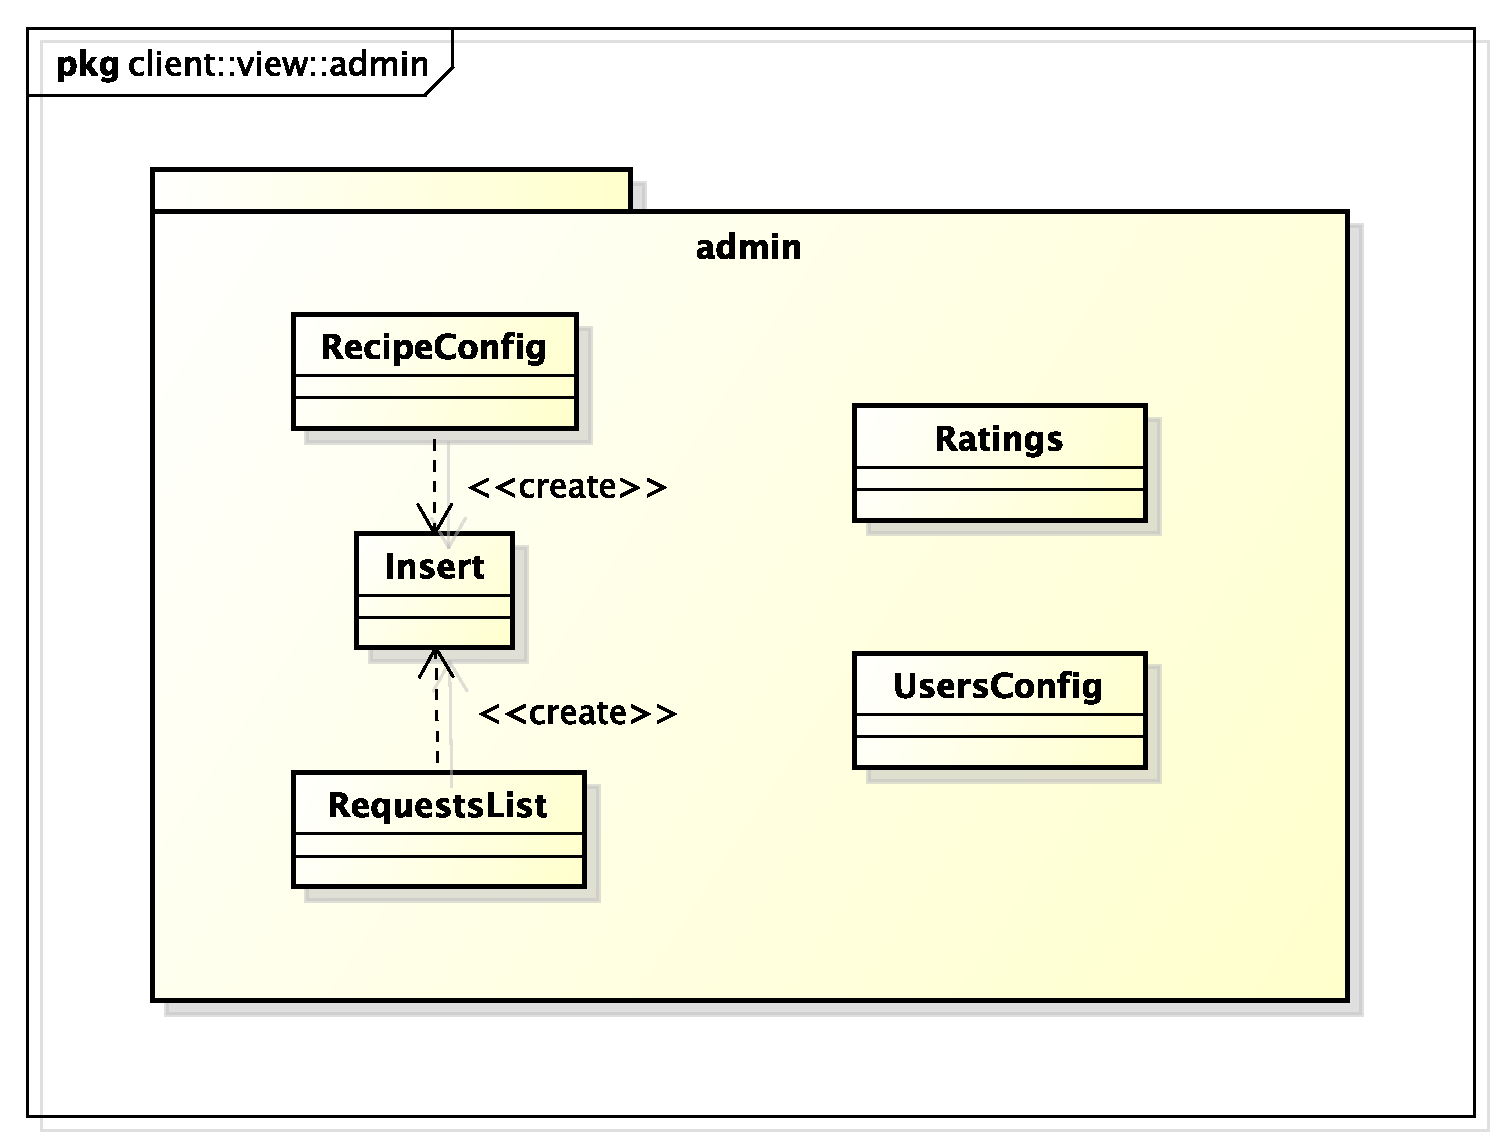
\includegraphics[scale=0.5]{./images/client_view_admin.pdf}}
	\caption{Package - client::view::admin}
\end{figure}

\begin{itemize}
	\item \textbf{Descrizione}: è il package che contiene tutte le pagine HTML che ha a disposizione l'utente che ha i privilegi di amministratore;\newline
	Per semplicità e chiarezza non è stato evidenziato nel grafico il fatto che ogni classe di questo package possiede un'istanza di MenuMain e di MenuSecondAdmin.
	\item \textbf{Padre}: client::view
	\item \textbf{Interazione con altri componenti}:
		\begin{itemize}
			\item client::controller::admin
		\end{itemize}
\end{itemize}

	\paragraph{Classi} % (fold)
		\subparagraph{bdsm\_app::client::view::admin::RecipeConfig} % (fold)
		\label{subp:bdsm_app_client_view_admin_recipeconfig}
			\begin{itemize}
				\item \textbf{Descrizione}: La classe rappresenta un template HTML per la visualizzazione dell'interfaccia di gestione delle Recipe;
				\item \textbf{Utilizzo}: Viene utilizzata per generare la pagina HTML della gestione delle Recipe;
				\item \textbf{Relazioni con altre classi}:
					\begin{itemize}
						\item client::view::user::MenuMain
						\item client::view::admin::MenuSecondAdmin
						\item client::view::admin::Insert
						\item client::controller::admin::RecipeConfigRoute
						\item client::controller::admin::RecipeConfigCtrl
					\end{itemize}
			\end{itemize}
		% subparagraph bdsm_app_client_view_admin_recipeconfig (end)

		\subparagraph{bdsm\_app::client::view::admin::RequestList} % (fold)
		\label{subp:bdsm_app_client_view_admin_requestlist}
			\begin{itemize}
				\item \textbf{Descrizione}: La classe rappresenta un template HTML per la visualizzazione della pagina di visione delle richieste di Recipe;
				\item \textbf{Utilizzo}: Viene utilizzata per generare la pagina HTML della lista delle richieste di Recipe;
				\item \textbf{Relazioni con altre classi}:
					\begin{itemize}
						\item client::view::user::MenuMain
						\item client::view::admin::MenuSecondAdmin
						\item client::view::admin::Insert
						\item client::controller::admin::RequestListRoute
						\item client::controller::admin::RequestListCtrl
					\end{itemize}
			\end{itemize}
		% subparagraph bdsm_app_client_view_admin_requestlist (end)

		\subparagraph{bdsm\_app::client::view::admin::Insert} % (fold)
		\label{subp:bdsm_app_client_view_admin_insert}
			\begin{itemize}
				\item \textbf{Descrizione}: La classe rappresenta un template HTML per la visualizzazione dell'interfaccia di inserimento di una nuova Recipe;
				\item \textbf{Utilizzo}: Viene utilizzata per generare la pagina HTML di inserimento di una nuova recipe;
				\item \textbf{Relazioni con altre classi}:
					\begin{itemize}
						\item client::view::user::MenuMain
						\item client::view::admin::MenuSecondAdmin
						\item client::view::admin::RecipeConfig
						\item client::view::admin::RequestList
						\item client::controller::admin::RecipeConfigRoute
						\item client::controller::admin::InsertRecipeCtrl
					\end{itemize}
			\end{itemize}
		% subparagraph bdsm_app_client_view_admin_insert (end)

		\subparagraph{bdsm\_app::client::view::admin::Ratings} % (fold)
		\label{subp:bdsm_app_client_view_admin_ratings}
			\begin{itemize}
				\item \textbf{Descrizione}: La classe rappresenta un template HTML per la visualizzazione della pagina dei voti assegnati alle varie Recipe;
				\item \textbf{Utilizzo}: Viene utilizzata per generare la pagina HTML di visione dei voti delle Recipe;
				\item \textbf{Relazioni con altre classi}:
					\begin{itemize}
						\item client::view::user::MenuMain
						\item client::view::admin::MenuSecondAdmin
						\item client::controller::admin::RatingsRoute
						\item client::controller::admin::RatingsCtrl
					\end{itemize}
			\end{itemize}
		% subparagraph bdsm_app_client_view_admin_ratings (end)

		\subparagraph{bdsm\_app::client::view::admin::UsersConfig} % (fold)
		\label{subp:bdsm_app_client_view_admin_usersconfig}
			\begin{itemize}
				\item \textbf{Descrizione}: La classe rappresenta un template HTML per la visualizzazione dell'interfaccia di gestione degli utenti;
				\item \textbf{Utilizzo}: Viene utilizzata per generare la pagina HTML di gestione degli utenti;
				\item \textbf{Relazioni con altre classi}:
					\begin{itemize}
						\item client::view::user::MenuMain
						\item client::view::admin::MenuSecondAdmin
						\item client::controller::admin::UsersConfigRoute
						\item client::controller::admin::UsersConfigCtrl
					\end{itemize}
			\end{itemize}
		% subparagraph bdsm_app_client_view_admin_usersconfig (end)

		\subparagraph{bdsm\_app::client::view::admin::MenuSecondAdmin} % (fold)
		\label{subp:bdsm_app_client_view_admin_menusecondadmin}
			\begin{itemize}
				\item \textbf{Descrizione}: La classe rappresenta un template HTML per la creazione del menù secondario di un utente amministratore;
				\item \textbf{Utilizzo}: Viene usata nel generare ogni pagina di un utente autenticato amministratore per generare il menù secondario;
				\item \textbf{Classi ereditate}:
					\begin{itemize}
						\item client::view::user::Menu
						\item client::view::user::MenuSecond
					\end{itemize}
				\item \textbf{Relazioni con altre classi}:
					\begin{itemize}
						\item client::view::user::Menu
						\item client::view::user::MenuSecond
						\item client::controller::admin::MenuSecondAdminCtrl
					\end{itemize}
			\end{itemize}
		% subparagraph bdsm_app_client_view_admin_menusecondadmin (end)

% subsubsection bdsm_app_client_view_admin (end) \clearpage \newpage
	% END PACKAGE VIEW

	% PACKAGE CONTROLLER
	% =================================================================================================
% File:			client_tier/controller.tex
% Description:	Defiinisce la sezione relativa al front-end dell'applicazione
% Created:		2015-04-07
% Author:		Tesser Paolo
% Email:		tesser.paolo@mashup-unipd.it
% =================================================================================================
% Modification History:
% Version		Modifier Date		Change											Author
% 0.0.1 		2015-04-07 			creato scheletro								Tesser Paolo
% =================================================================================================
% 0.0.2			2015-04-07			scheletro delle classi dei pack					Tesser Paolo
% ================================================================================================
% 0.0.3			2015-04-08			descrizioni classi del pack controller_public	Tesser Paolo
% ================================================================================================
% 0.0.4			2015-04-08			inserite relazioni tra le classi				Tesser Paolo
% ================================================================================================
% 0.0.5			2015-04-09			completata descrizione classi					Tesser Paolo
% ================================================================================================
%

% CONTENUTO DEL CAPITOLO

\subsubsection{client::controller} % (fold)
\label{ssub:bdsm_app_client_controller}
Le classi definite per la gestione dell'indirizzamento delle pagine HTML dell'applicazione, e cioè quelle terminanti con \textbf{Route}, rappresentano delle configurazioni. Questo implica che non possiedono metodi o attributi, ma al massimo utilizzano servizi per attuare il loro compito che vengono descritti nella nota introduttiva in \ref{sub:client}. La zona quindi dedicata a quei valori sarà marcata come specificato in \ref{sub:note_specifica} e non verrà fornita nessuna immagine.


\begin{figure}[htbp]
	\centering
	\centerline{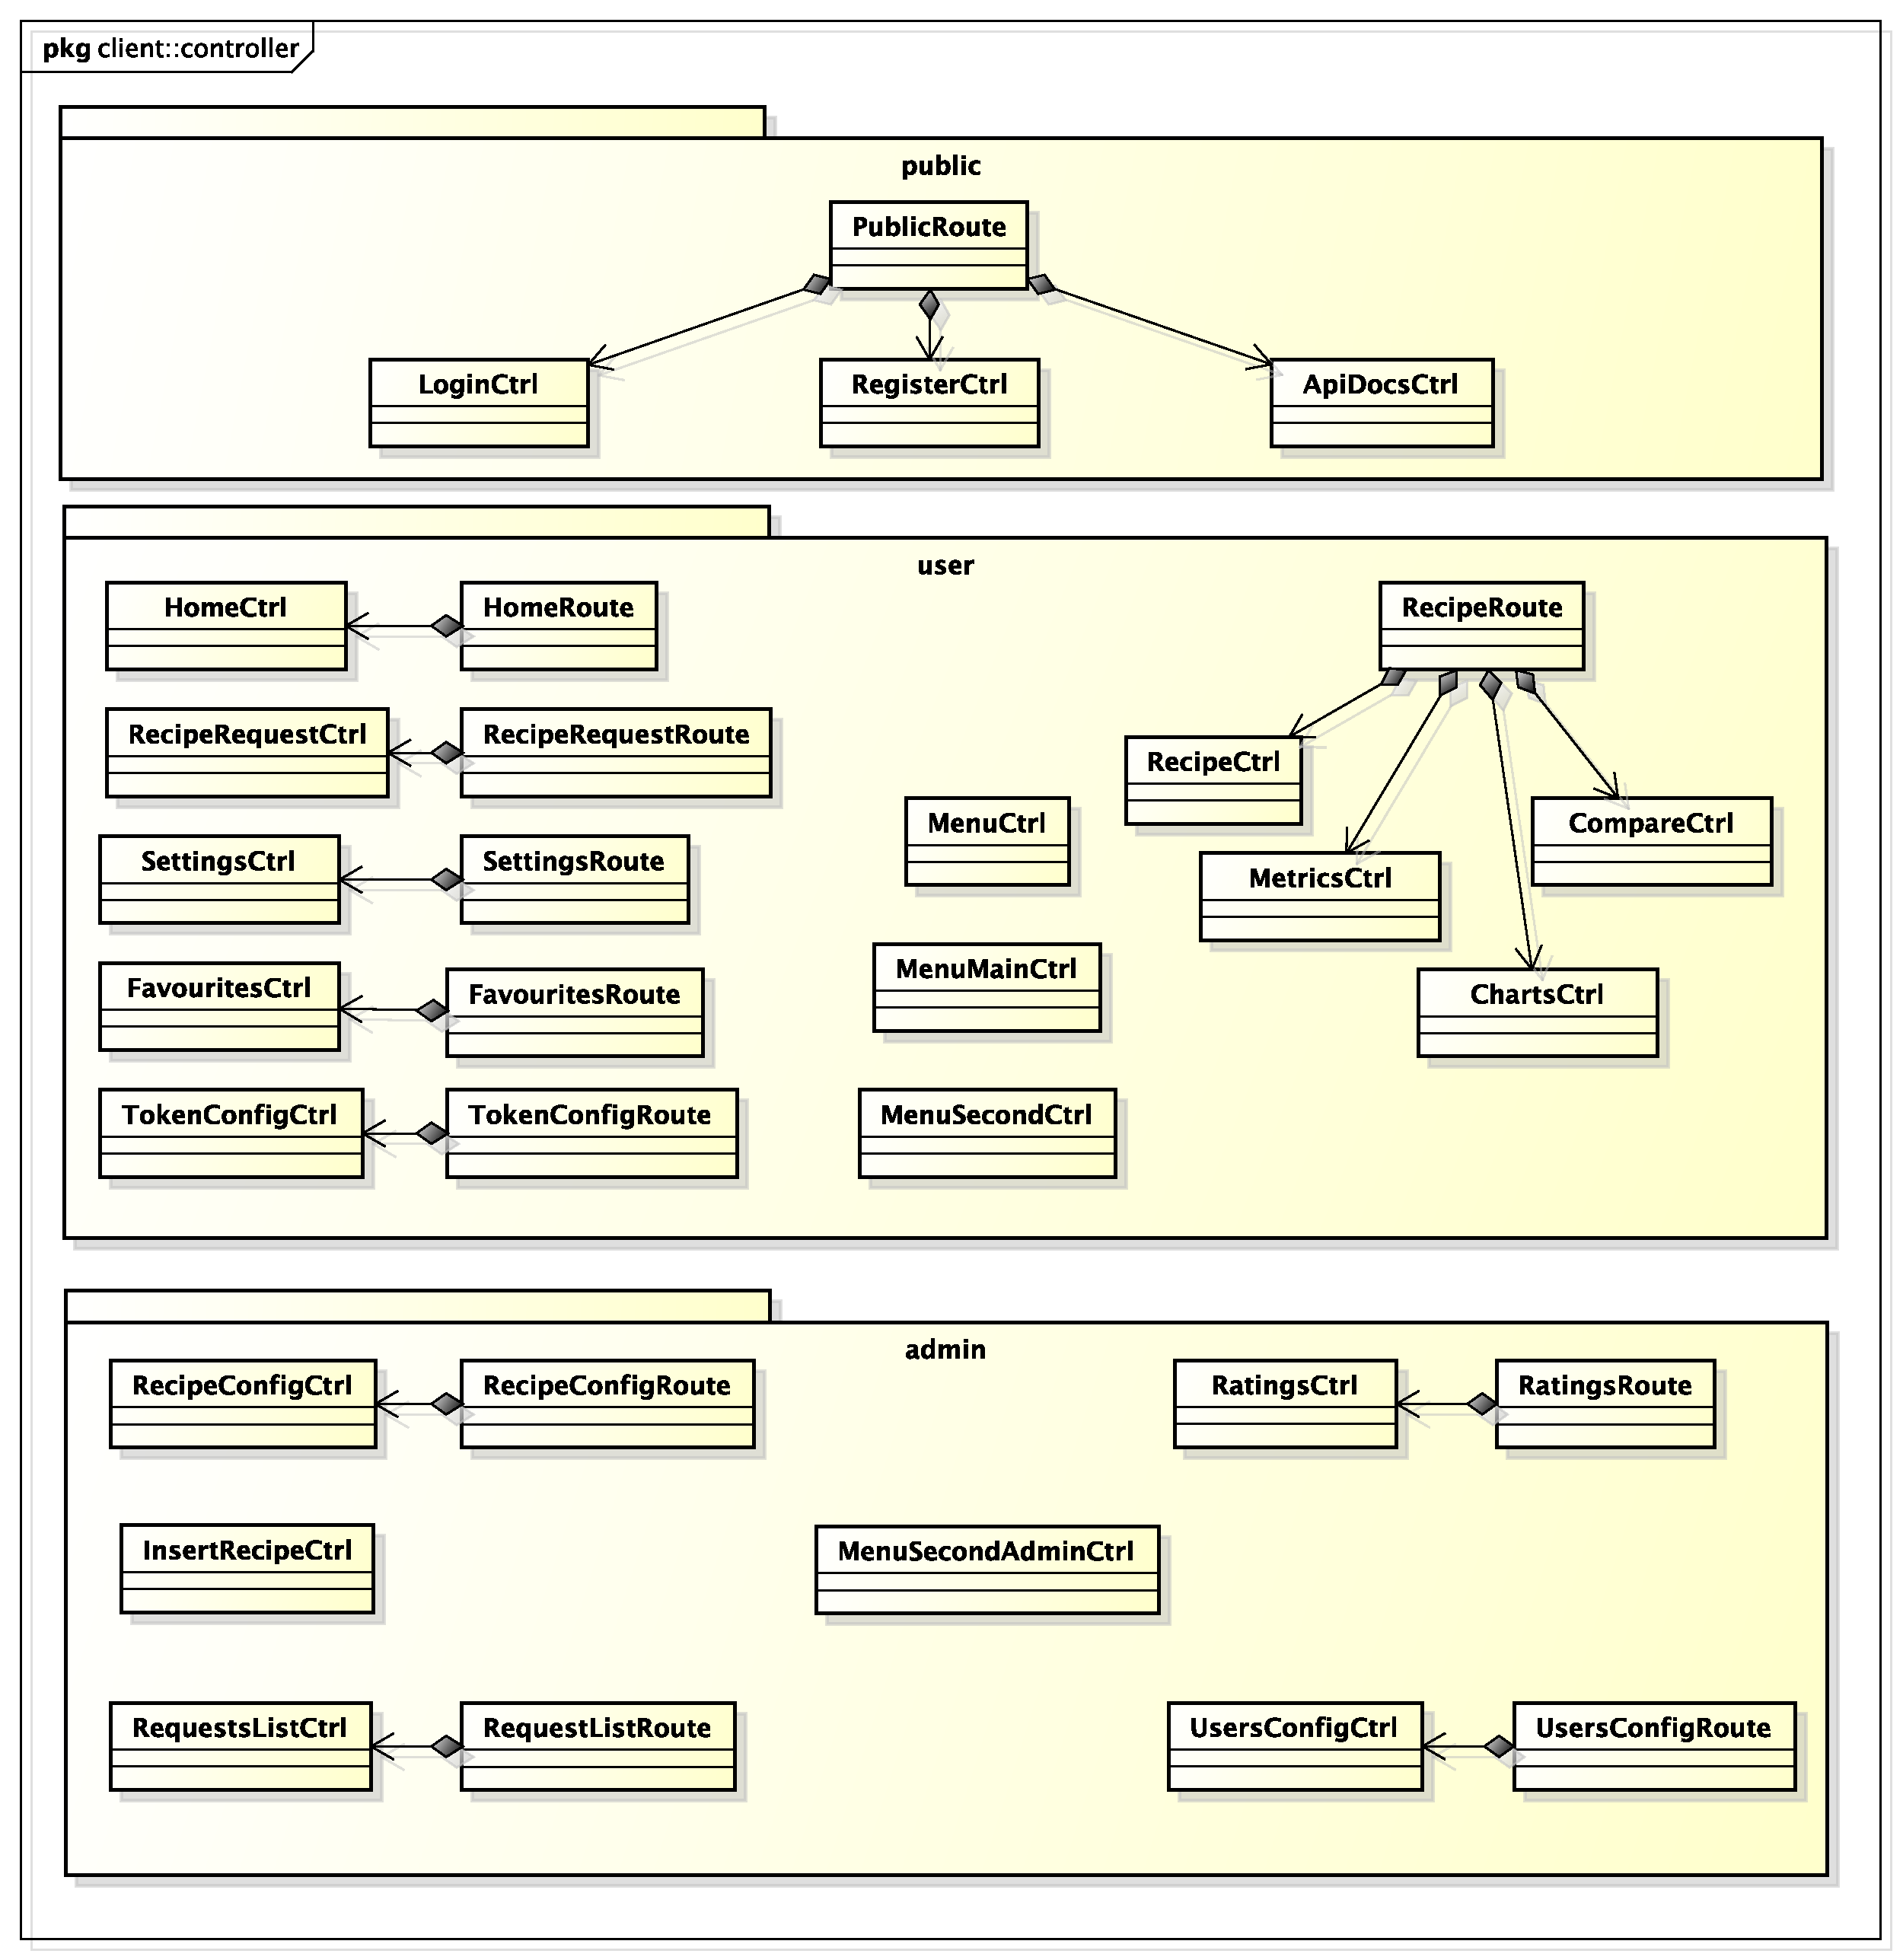
\includegraphics[scale=0.4]{./images/client/client_controller.pdf}}
	\caption{Package - client::controller}
\end{figure}

\begin{itemize}
	\item \textbf{Descrizione}: è il package che contiene le componenti che contengono i controller dell'applicazione e che incapsulano le funzionalità di two-way data binding tra le View e il Model. In esse è contenuta la logica applicativa riguardante le diverse pagine HTML;
	\item \textbf{Padre}: client;
	\item \textbf{Package contenuti}:
		\begin{itemize}
			\item client::controller::public
			\item client::controller::user
			\item client::controller::admin
		\end{itemize}
	\item \textbf{Interazione con altri componenti}:
		\begin{itemize}
			\item client::model
			\item client::view
		\end{itemize}
\end{itemize}
% subsubsection bdsm_app_client_controller (end)


\subsubsection{client::controller::public} % (fold)
\label{ssub:bdsm_app_client_controller_public}
\begin{figure}[htbp]
	\centering
	\centerline{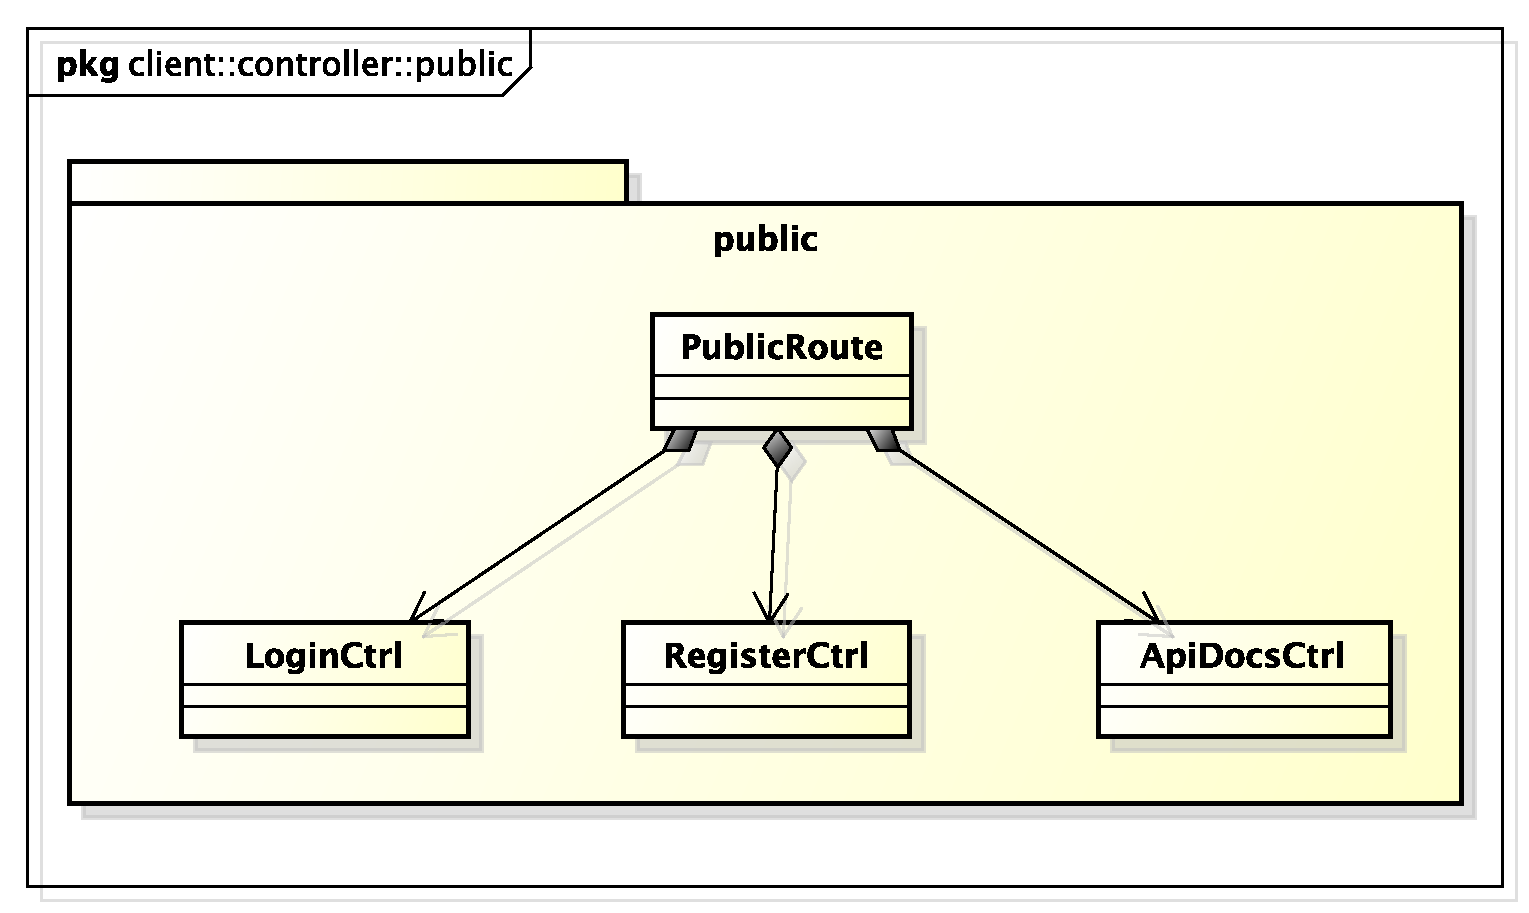
\includegraphics[scale=0.6]{./images/client/client_controller_public.pdf}}
	\caption{Package - client::controller::public}
\end{figure}

\begin{itemize}
	\item \textbf{Descrizione}: è il package che contiene le classi che controllano le decisioni di che pagine HTML mostrare all'utente che non si è ancora autenticato e di quali operazioni poter effettuare su di esse;
	\item \textbf{Padre}: client::controller
	\item \textbf{Interazione con altri componenti}:
		\begin{itemize}
			\item client::model::public
			\item client::view::public
		\end{itemize}
\end{itemize}

	\paragraph{Classi} % (fold)
		\subparagraph{client::controller::public::PublicRoute} % (fold)
		\label{subp:bdsm_app_client_controller_public_publicrouteconfig}

		\begin{itemize}
			\item \textbf{Descrizione}: la classe serve a gestire l'indirizzamento e l'assegnazione di uno stato al template HTML riguardante le pagine che può visualizzare un utente non autenticato, quali quella di autenticazione, di registrazione o di visione della documentazione dei servizi REST offerti;
			\item \textbf{Utilizzo}: viene utilizzata per reindirizzare l'utente al template HTML adeguato in caso si voglia o autenticare o registrare al sistema, o visualizzare i servizi REST offerti, ed assegnare al template scelto il controller opportuno per gestire i diversi compiti. Nel caso l'utente fosse già autenticato, la classe provvederà a reindirizzarlo all'URL associato alla Home;
			\item \textbf{Relazioni con altre classi}:
				\begin{itemize}
					\item client::view::public::Login
					\item client::view::public::Register
					\item client::view::public::ApiDocs
					\item client::controller::public::LoginCtrl
					\item client::controller::public::RegisterCtrl
					\item client::controller::public::ApiDocsCtrl
				\end{itemize}
				\item \textbf{Attributi associati allo \$scope}: N/A
				\item \textbf{Metodi associati allo \$scope e privati}: N/A
				\item \textbf{Servizi AngularJS utilizzati}:
					\begin{itemize}
						\item \$stateProvider
					\end{itemize}
		\end{itemize}
		% subparagraph bdsm_app_client_controller_public_publicrouteconfig (end)

		\subparagraph{client::controller::public::LoginCtrl} % (fold)
		\label{subp:bdsm_app_client_controller_public_loginctrl}
			\begin{figure}[htbp]
				\centering
				\centerline{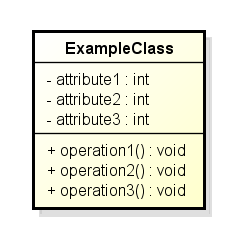
\includegraphics[scale=0.7]{./images/client/classes/example_class.png}}
				\caption{Classe - client::controller::public::LoginCtrl}
			\end{figure}
			\begin{itemize}
				\item \textbf{Descrizione}: la classe è il controller che serve a gestire la logica applicativa riguardante l'autenticazione al sistema;
				\item \textbf{Utilizzo}: viene utilizzata per gestire le operazioni di autenticazione al sistema qualora un utente non autenticato decidesse di effettuare l'accesso. Richiamando quindi i servizi che mettono in comunicazione il client con il server, verifica le credenziali ed effettua un reindirizzamento alla Home qualora fossero valide;
				\item \textbf{Relazioni con altre classi}:
					\begin{itemize}
						\item client::model::services::AuthService
						\item client::view::public::Login
						\item client::controller::public::PublicRoute
					\end{itemize}

				\item \textbf{Attributi associati allo \$scope}:
					\begin{itemize}

						\item \textcolor{forestgreen}{\texttt{+ credentials : oggetto JSON}}
							\begin{description}
								\item \textbf{Descrizione}: oggetto nel formato JSON che contiene il valore iniziale dei campi mail e password che inizialmente saranno vuoti.
							\end{description}

					\end{itemize}

				\item \textbf{Metodi associati allo \$scope e privati}:
					\begin{itemize}
						\item \textcolor{forestgreen}{\texttt{+ login(cred)}}
							\begin{description}
								\item \textbf{Descrizione}: gli vengono passati i dati dalla view e viene invocato il metodo login della classe AuthService.
							\end{description}

					\end{itemize}

				\item \textbf{Servizi AngularJS utilizzati}: N/A

			\end{itemize}
		% subparagraph bdsm_app_client_controller_public_loginctrl (end)

		\subparagraph{client::controller::public::RegisterCtrl} % (fold)
		\label{subp:bdsm_app_client_controller_public_registerctrl}
			\begin{figure}[htbp]
				\centering
				\centerline{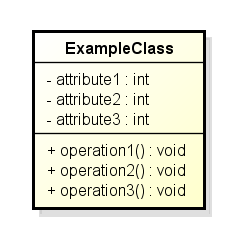
\includegraphics[scale=0.7]{./images/client/classes/example_class.png}}
				\caption{Classe - client::controller::public::RegisterCtrl}
			\end{figure}
			\begin{itemize}
				\item \textbf{Descrizione}: la classe è il controller che serve a gestire la logica applicativa riguardante la registrazione al sistema;
				\item \textbf{Utilizzo}: viene utilizzata per gestire le operazioni di registrazione al sistema qualora un utente che non si è ancora registrato decidesse di effettuare l'accesso. Richiamando quindi i servizi che mettono in comunicazione il client con il server, verifica le credenziali ed effettua un reindirizzamento alla pagina di Login qualora la registrazione fosse avvenuta con successo;
				\item \textbf{Relazioni con altre classi}:
					\begin{itemize}
						\item client::model::services::AuthService
						\item client::model::data::UserMode
						\item client::view::public::Register
						\item client::controller::public::PublicRoute
					\end{itemize}
				\item \textbf{Attributi associati allo \$scope}:
					\begin{itemize}
						\item \textcolor{forestgreen}{\texttt{+ credentials : oggetto JSON}}
							\begin{description}
								\item \textbf{Descrizione}: oggetto nel formato JSON che contiene il valore iniziale dei campi username, mail, password e password da confermare che inizialmente saranno vuoti.
							\end{description}

						\item \textcolor{forestgreen}{\texttt{+ matchPwd : bool}} 
							\begin{description}
								\item \textbf{Descrizione}: booleano inizializzato a false che cambia valore se il valore della nuova password e quello di conferma non combaciano.
							\end{description}

					\end{itemize}

				\item \textbf{Metodi associati allo \$scope e privati}:
					\begin{itemize}
						\item \textcolor{forestgreen}{\texttt{+ register(cred)}}
							\begin{description}
								\item \textbf{Descrizione}: gli vengono passati i dati dalla view e viene invocato il metodo register della classe AuthService.
							\end{description}

						\item \textcolor{forestgreen}{\texttt{- checkMatchPwd(newPwd, confirmNewPwd)}}
							\begin{description}
								\item \textbf{Descrizione}: gli vengono passati i dati dalla view e viene invocato il metodo register della classe AuthService.
							\end{description}
					\end{itemize}

				\item \textbf{Servizi AngularJS utilizzati}: N/A

			\end{itemize}
		% subparagraph bdsm_app_client_controller_public_registerctrl (end)

		\subparagraph{client::controller::public::ApiDocsCtrl} % (fold)
		\label{subp:bdsm_app_client_controller_public_apidocsctrl}
			\begin{figure}[htbp]
				\centering
				\centerline{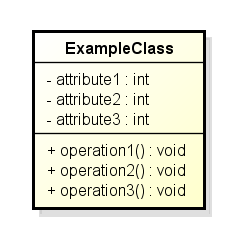
\includegraphics[scale=0.7]{./images/client/classes/example_class.png}}
				\caption{Classe - client::controller::public::ApiDocsCtrl}
			\end{figure}
		\begin{itemize}
			\item \textbf{Descrizione}: la classe è il controller che serve a gestire la logica applicativa riguardante la pagina di visualizzazione dei servizi REST che il sistema offre;
			\item \textbf{Utilizzo}: viene utilizzata per gestire in maniera automatica la documentazione riguardante i servizi REST offerti dal sistema;
			\item \textbf{Relazioni con altre classi}:
				\begin{itemize}
					\item client::model::ApiDocsModel
					\item client::view::public::ApiDocs
					\item client::controller::public::PublicRoute
				\end{itemize}

			\item \textbf{Attributi associati allo \$scope}:
				\begin{itemize}
					\item \textcolor{forestgreen}{\texttt{+ restServices : array di oggetti JSON }}
						\begin{description}
							\item \textbf{Descrizione}: array di oggetti nel formato JSON che rappresentano la lista delle API pubbliche. Questa variabile viene inizializzata tramite la chiamata immediata alla funzione privata getRestService.
						\end{description}
				\end{itemize}

			\item \textbf{Metodi associati allo \$scope e privati}:
				\begin{itemize}
					\item \textcolor{forestgreen}{\texttt{- getRestService()}}
						\begin{description}
							\item \textbf{Descrizione}: funzione che preleva la lista delle API pubbliche tramite una chiamata alla classe ApiDocsModel.
						\end{description}
				\end{itemize}

			\item \textbf{Servizi AngularJS utilizzati}: N/A

		\end{itemize}
		% subparagraph bdsm_app_client_controller_public_apidocsctrl (end)


% subsubsection bdsm_app_client_controller_public (end)



\subsubsection{client::controller::user} % (fold)
\label{ssub:bdsm_app_client_controller_user}
\begin{figure}[htbp]
	\centering
	\centerline{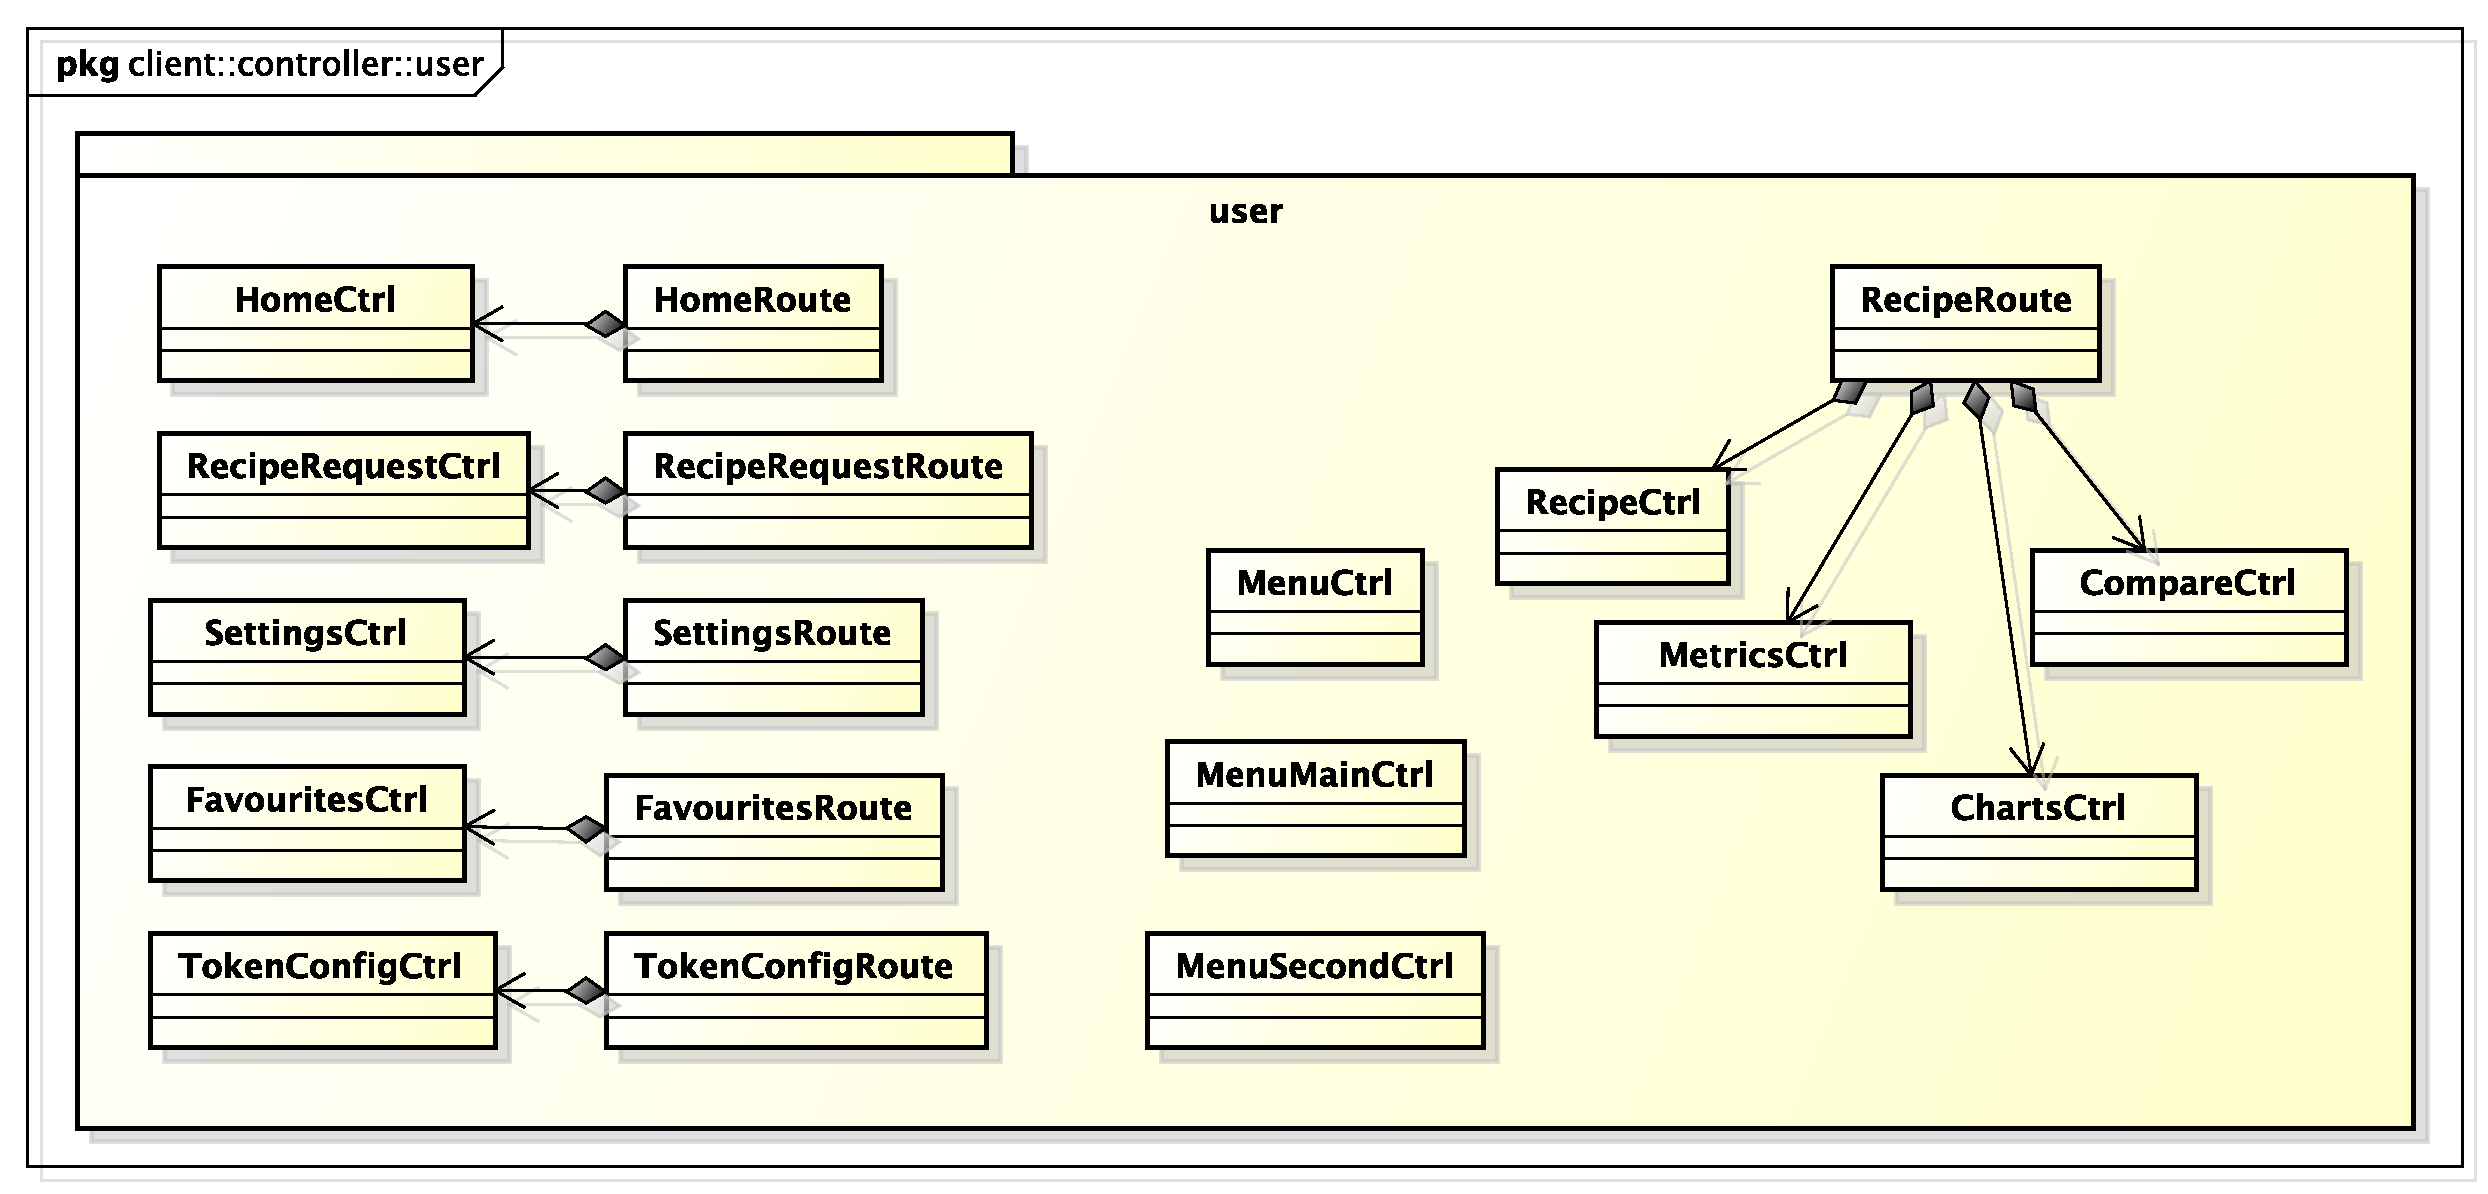
\includegraphics[scale=0.45]{./images/client/client_controller_user.pdf}}
	\caption{Package - client::controller::user}
\end{figure}

\begin{itemize}
	\item \textbf{Descrizione}: è il package che contiene le classi che controllano le decisioni di che pagine HTML mostrare all'utente autenticato e di quali operazioni poter effettuare su di esse;
	\item \textbf{Padre}: client::controller
	\item \textbf{Interazione con altri componenti}:
		\begin{itemize}
			\item client::model::user
			\item client::view::user
		\end{itemize}
\end{itemize}

	\paragraph{Classi} % (fold)
		\subparagraph{client::controller::user::MenuCtrl} % (fold)
		\label{subp:client_controller_user_menuctrl}

			\begin{itemize}
				\item \textbf{Descrizione}: la classe è il controller che serve a gestire la logica applicativa riguardante la parte in comune tra i diversi menu presenti nell'applicazione
				\item \textbf{Utilizzo}: viene utilizzata per gestire le operazioni in comune e gli stati tra i diversi menu effettivi che conterranno i vari collegamenti alle diverse pagine;
				\item \textbf{Relazioni con altre classi}:
					\begin{itemize}
						\item client::view::user::Menu
					\end{itemize}
				\item \textbf{Attributi associati allo \$scope}: N/A
				\item \textbf{Metodi associati allo \$scope e privati}: N/A
			\end{itemize}
		% subparagraph client_controller_user_menuctrl (end)

		\subparagraph{client::controller::user::MenuMainCtrl} % (fold)
		\label{subp:client_controller_user_menumainctrl}

			\begin{itemize}
				\item \textbf{Descrizione}: la classe è il controller che serve a gestire la logica applicativa riguardante il menu principale dell'applicazione;
				\item \textbf{Utilizzo}: viene utilizzata per gestire i collegamenti principali ad alcune pagine del sistema ed ad effettuare l'operazione di logout;
				\item \textbf{Classi ereditate}:
					\begin{itemize}
						\item client::controller::user::MenuCtrl. Questa ereditarietà è solo logica e non viene implementata in nessuna forma.
					\end{itemize}
				\item \textbf{Relazioni con altre classi}:
					\begin{itemize}
						\item client::view::user::MenuMain
						\item client::controller::user::LogoutCtrl
						\item client::controller::public::HomeRoute
						\item client::controller::user::SettingsRoute
					\end{itemize}
				\item \textbf{Attributi associati allo \$scope}: N/A
				\item \textbf{Metodi associati allo \$scope e privati}: N/A
			\end{itemize}
		% subparagraph client_controller_user_menumainctrl (end)

		\subparagraph{client::controller::user::MenuSecondCtrl} % (fold)
		\label{subp:client_controller_user_menusecondctrl}

			\begin{itemize}
				\item \textbf{Descrizione}: la classe è il controller che serve a gestire la logica applicativa riguardante il menu secondario dell'applicazione;
				\item \textbf{Utilizzo}: viene utilizzata per gestire i collegamenti secondari alla maggior parte delle pagine del sistema;
				\item \textbf{Classi ereditate}:
					\begin{itemize}
						\item client::controller::user::MenuCtrl. Questa ereditarietà è solo logica e non viene implementata in nessuna forma.
					\end{itemize}
				\item \textbf{Relazioni con altre classi}:
					\begin{itemize}
						\item client::view::user::MenuSecond
						\item client::controller::user::RecipeRoute
						\item client::controller::user::RecipeRequestRoute
						\item client::controller::user::FavouritesRoute
						\item client::controller::user::TokenConfigRoute
					\end{itemize}
				\item \textbf{Attributi associati allo \$scope}: N/A
				\item \textbf{Metodi associati allo \$scope e privati}: N/A
			\end{itemize}
		% subparagraph client_controller_user_menusecondctrl (end)


		\subparagraph{client::controller::user::HomeRoute} % (fold)
		\label{subp:bdsm_app_client_controller_user_homerouteconfig}
			\begin{itemize}
				\item \textbf{Descrizione}: la classe serve a gestire l'indirizzamento e l'assegnazione di uno stato al template HTML riguardante la Home page dell'utente che ha effettuato l'accesso al sistema;
				\item \textbf{Utilizzo}: viene utilizzata per reindirizzare l'utente al template HTML della pagina iniziale dell'applicativo una volta effettuato l'accesso ed assegnare al template scelto il controller opportuno per gestire i diversi compiti;
				\item \textbf{Relazioni con altre classi}:
					\begin{itemize}
						\item client::view::user::Home
						\item client::controller::user::HomeCtrl
					\end{itemize}
				\item \textbf{Attributi associati allo \$scope}: N/A
				\item \textbf{Metodi associati allo \$scope e privati}: N/A
				\item \textbf{Servizi AngularJS utilizzati}:
					\begin{itemize}
						\item \$stateProvider
					\end{itemize}
			\end{itemize}
		% subparagraph bdsm_app_client_controller_user_homerouteconfig (end)

		\subparagraph{client::controller::user::HomeCtrl} % (fold)
		\label{subp:client_controller_user_homectrl}
			\begin{figure}[htbp]
				\centering
				\centerline{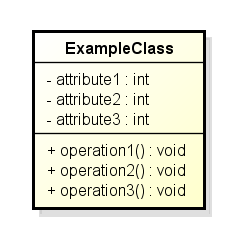
\includegraphics[scale=0.7]{./images/client/classes/example_class.png}}
				\caption{Classe - client::controller:user::HomeCtrl}
			\end{figure}
			\begin{itemize}
				\item \textbf{Descrizione}: la classe è il controller che serve a gestire la logica applicativa riguardante la pagina principale dell'applicazione, una volta che l'utente ha effettuato l'accesso;
				\item \textbf{Utilizzo}: viene utilizzata per gestire la pagina principale dell'applicazione. Su di essa per il momento non sono state previste particolari operazioni, ma viene lo stesso inserito un controller per scopi futuri;
				\item \textbf{Relazioni con altre classi}:
					\begin{itemize}
						\item client::view::user::Home
						\item client::controller::user::HomeRoute
					\end{itemize}

				\item \textbf{Attributi associati allo \$scope}: N/A
				\item \textbf{Metodi associati allo \$scope e privati}: N/A
				\item \textbf{Servizi AngularJS utilizzati}: N/A

			\end{itemize}
		% subparagraph client_controller_user_homectrl (end)

		\subparagraph{client::controller::user::RecipeRoute} % (fold)
		\label{subp:bdsm_app_client_controller_user_reciperouteconfig}

			\begin{itemize}
				\item \textbf{Descrizione}: la classe serve a gestire l'indirizzamento e l'assegnazione di uno stato al template HTML riguardante la pagina delle Recipe e di quelle che vengono create da essa, quali \textbf{Metrics}, \textbf{Charts} e \textbf{Compare};
				\item \textbf{Utilizzo}: viene utilizzata per reindirizzare l'utente al template HTML della pagina relativa alle Recipe presenti nel sistema ed assegnare al template scelto il controller opportuno per gestire i diversi compiti.  Da li l'utente potrà muoversi a seconda delle sue esigenze nelle pagine citate nella \emph{Descrizione};
				\item \textbf{Relazioni con altre classi}:
					\begin{itemize}
						\item client::view::user::Recipe
						\item client::view::user::Metrics
						\item client::view::user::Charts
						\item client::view::user::Compare
						\item client::controller::user::RecipeCtrl
						\item client::controller::user::MetricsCtrl
						\item client::controller::user::ChartsCtrl
						\item client::controller::user::CompareCtrl
					\end{itemize}
				\item \textbf{Attributi associati allo \$scope}: N/A
				\item \textbf{Metodi associati allo \$scope e privati}: N/A
				\item \textbf{Servizi AngularJS utilizzati}:
					\begin{itemize}
						\item \$stateProvider
					\end{itemize}
			\end{itemize}
		% subparagraph bdsm_app_client_controller_user_reciperouteconfig (end)

		\subparagraph{client::controller::user::RecipeCtrl} % (fold)
		\label{subp:client_controller_user_recipectrl}
			\begin{figure}[htbp]
				\centering
				\centerline{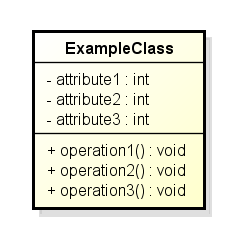
\includegraphics[scale=0.7]{./images/client/classes/example_class.png}}
				\caption{Classe - client::controller:user::RecipeCtrl}
			\end{figure}
			\begin{itemize}
				\item \textbf{Descrizione}: la classe è il controller che serve a gestire la logica applicativa riguardante le Recipe presenti nel sistema;
				\item \textbf{Utilizzo}: viene utilizzata per gestire la lista delle Recipe disponibili che verranno mostrate all'utente e le operazioni che esso ha a disposizione su queste. Queste operazioni saranno sotto forma di pulsanti associati a ciascuna metrica che porteranno l'utente o a visualizzare tutte le metriche inerenti alla Recipe scelta o ad effettuare un confronto tra le diverse metriche presenti;
				\item \textbf{Relazioni con altre classi}:
					\begin{itemize}
						\item client::model::services::RecipeService
						\item client::view::user::Recipe
						\item client::controller::view::RecipeRoute
					\end{itemize}

				\item \textbf{Attributi associati allo \$scope}:
					\begin{itemize}
						\item \textcolor{forestgreen}{\texttt{ + listRecipes : array di oggetti JSON}}
							\begin{description}
								\item \textbf{Descrizione}: array di oggetti nel formato JSON che rappresentano la lista delle recipe presenti nel sistema. Questa variabile viene inizializzata tramite la chiamata immediata al metodo privata getListOfRecipes. Il formato degli oggetti JSON contenuti nell'array è il seguente:
								\begin{verbatim}
									{
									    id: '42',
									    title: 'Titolo della Recipe',
									    desc: 'Descrizione della Recipe'
									}
								\end{verbatim}
							\end{description}

					\end{itemize}

				\item \textbf{Metodi associati allo \$scope e privati}:
					\begin{itemize}
						\item \textcolor{forestgreen}{\texttt{- getListOfRecipes()}}
							\begin{description}
								\item \textbf{Descrizione}: metodo che preleva la lista delle recipe tramite una chiamata al metodo \textbf{getRecipesList} della classe RecipeService.
							\end{description}

					\end{itemize}

				\item \textbf{Servizi AngularJS utilizzati}: N/A

			\end{itemize}
		% subparagraph client_controller_user_recipectrl (end)

		\subparagraph{client::controller::user::MetricsCtrl} % (fold)
		\label{subp:client_controller_user_metricsctrl}
			\begin{figure}[htbp]
				\centering
				\centerline{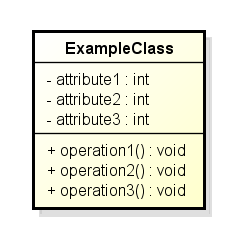
\includegraphics[scale=0.7]{./images/client/classes/example_class.png}}
				\caption{Classe - client::controller:user::MetricsCtrl}
			\end{figure}
			\begin{itemize}
				\item \textbf{Descrizione}: la classe è il controller che serve a gestire la logica applicativa riguardante le metriche associate ad una Recipe precisa;
				\item \textbf{Utilizzo}: viene utilizzata per gestire la lista delle metriche associate a una Recipe, fornendo dei pulsanti per ciascuna che serviranno all'utente per andare a visualizzare i grafici inerenti alla metrica selezionata;
				\item \textbf{Relazioni con altre classi}:
					\begin{itemize}
						\item client::model::services::RecipeService
						\item client::view::user::metrics
						\item client::controller::user::RecipeRoute
					\end{itemize}

				\item \textbf{Attributi associati allo \$scope}:
					\begin{itemize}
						\item \textcolor{forestgreen}{\texttt{+ titleRecipe : String}}
							\begin{description}
								\item \textbf{Descrizione}: parametro che identifica il nome della Recipe che contiene le metriche visualizzate dalla pagina.
							\end{description}
						\item \textcolor{forestgreen}{\texttt{+ titleRecipe : String}}
							\begin{description}
								\item \textbf{Descrizione}: parametro che identifica il nome della Recipe che contiene le metriche visualizzate dalla pagina.
							\end{description}
						\item \textcolor{forestgreen}{\texttt{+ titleRecipe : String}}
							\begin{description}
								\item \textbf{Descrizione}: parametro che identifica il nome della Recipe che contiene le metriche visualizzate dalla pagina.
							\end{description}
						\item \textcolor{forestgreen}{\texttt{+ titleRecipe : String}}
							\begin{description}
								\item \textbf{Descrizione}: parametro che identifica il nome della Recipe che contiene le metriche visualizzate dalla pagina.
							\end{description}
						\item \textcolor{forestgreen}{\texttt{+ titleRecipe : String}}
							\begin{description}
								\item \textbf{Descrizione}: parametro che identifica il nome della Recipe che contiene le metriche visualizzate dalla pagina.
							\end{description}

					\end{itemize}

				\item \textbf{Metodi associati allo \$scope e privati}:
					\begin{itemize}
						\item \textcolor{forestgreen}{\texttt{TODO}}
							\begin{description}
								\item \textbf{Descrizione}: TODO
							\end{description}

					\end{itemize}

				\item \textbf{Servizi AngularJS utilizzati}:
					\begin{itemize}
						\item \$stateParams
					\end{itemize}

			\end{itemize}
		% subparagraph client_controller_user_metricsctrl (end)

		\subparagraph{client::controller::user::ChartsCtrl} % (fold)
		\label{subp:client_controller_user_chartsctrl}
			\begin{figure}[htbp]
				\centering
				\centerline{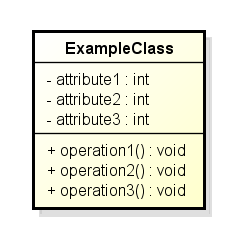
\includegraphics[scale=0.7]{./images/client/classes/example_class.png}}
				\caption{Classe - client::controller:user::ChartsCtrl}
			\end{figure}
			\begin{itemize}
				\item \textbf{Descrizione}: la classe è il controller che serve a gestire la logica applicativa riguardante i grafici che vengono generati a partire dai dati associati ad una metrica precisa;
				\item \textbf{Utilizzo}: viene utilizzata per gestire e generare i grafici a partire dai dati della metrica selezionata. La classe richiamerà i diversi metodi presenti nel \textbf{model} che a seconda della tipologia della metrica, creeranno i grafici opportuni;
				\item \textbf{Relazioni con altre classi}:
					\begin{itemize}
						\item client::model::services::RecipeService
						\item client::view::user::Charts
						\item client::controller::user::RecipeRoute
					\end{itemize}

				\item \textbf{Attributi associati allo \$scope}:
					\begin{itemize}
						\item \textcolor{forestgreen}{\texttt{TODO}}
							\begin{description}
								\item \textbf{Descrizione}: TODO
							\end{description}

					\end{itemize}

				\item \textbf{Metodi associati allo \$scope e privati}:
					\begin{itemize}
						\item \textcolor{forestgreen}{\texttt{TODO}}
							\begin{description}
								\item \textbf{Descrizione}: TODO
							\end{description}

					\end{itemize}

				\item \textbf{Servizi AngularJS utilizzati}:
					\begin{itemize}
						\item TODO
					\end{itemize}

			\end{itemize}
		% subparagraph client_controller_user_chartsctrl (end)

		\subparagraph{client::controller::user::CompareCtrl} % (fold)
		\label{subp:client_controller_user_comparectrl}
			\begin{figure}[htbp]
				\centering
				\centerline{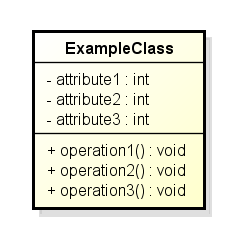
\includegraphics[scale=0.7]{./images/client/classes/example_class.png}}
				\caption{Classe - client::controller:user::CompareCtrl}
			\end{figure}
			\begin{itemize}
				\item \textbf{Descrizione}: la classe è il controller che serve a gestire la logica applicativa riguardante la generazione di confronti tra diverse metriche di una Recipe;
				\item \textbf{Utilizzo}: viene utilizzata per gestire e generare i grafici a partire dai dati delle metriche selezionate che si vuole confrontare;
				\item \textbf{Relazioni con altre classi}:
					\begin{itemize}
						\item client::model::data::CompareModel
						\item client::view::user::Compare
						\item client::controller::RecipeRoute
					\end{itemize}

				\item \textbf{Attributi associati allo \$scope}:
					\begin{itemize}
						\item \textcolor{forestgreen}{\texttt{TODO}}
							\begin{description}
								\item \textbf{Descrizione}: TODO
							\end{description}

					\end{itemize}

				\item \textbf{Metodi associati allo \$scope e privati}:
					\begin{itemize}
						\item \textcolor{forestgreen}{\texttt{TODO}}
							\begin{description}
								\item \textbf{Descrizione}: TODO
							\end{description}

					\end{itemize}

				\item \textbf{Servizi AngularJS utilizzati}:
					\begin{itemize}
						\item TODO
					\end{itemize}

			\end{itemize}
		% subparagraph client_controller_user_comparectrl (end)

		\subparagraph{client::controller::user::RecipeRequestRoute} % (fold)
		\label{subp:bdsm_app_client_controller_user_reciperequestrouteconfig}
			\begin{itemize}
				\item \textbf{Descrizione}: la classe serve a gestire l'indirizzamento e l'assegnazione di uno stato al template HTML riguardante la pagina che serve ad un utente per generare delle richieste di nuove Recipe da inserire nel sistema;
				\item \textbf{Utilizzo}: viene utilizzata per reindirizzare l'utente al template HTML della pagina che permette all'utente di fare delle richieste per delle nuove Recipe ed assegnare al template scelto il controller opportuno per gestire i diversi compiti;
				\item \textbf{Relazioni con altre classi}:
					\begin{itemize}
						\item client::view::user::RecipeRequest
						\item client::controller::user::RecipeRequestCtrl
					\end{itemize}
				\item \textbf{Attributi associati allo \$scope}: N/A
				\item \textbf{Metodi associati allo \$scope e privati}: N/A
				\item \textbf{Servizi AngularJS utilizzati}:
					\begin{itemize}
						\item \$stateProvider
					\end{itemize}
			\end{itemize}
		% subparagraph bdsm_app_client_controller_user_reciperequestrouteconfig (end)

		\subparagraph{client::controller::user::RecipeRequestCtrl} % (fold)
		\label{subp:client_controller_user_reciperequestctrl}
			\begin{figure}[htbp]
				\centering
				\centerline{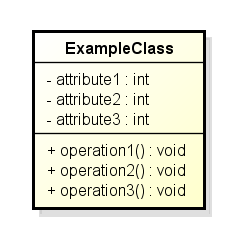
\includegraphics[scale=0.7]{./images/client/classes/example_class.png}}
				\caption{Classe - client::controller:user::RecipeRequestCtrl}
			\end{figure}
			\begin{itemize}
				\item \textbf{Descrizione}: la classe è il controller che serve a gestire la logica applicativa riguardante il form che l'utente deve compilare per effettuare una richiesta per una nuova Recipe;
				\item \textbf{Utilizzo}: viene utilizzata per gestire il form che l'utente, che desidera fare richiesta per l'inserimento di una nuova Recipe, deve compilare. La classe dovrà utilizzare il verificare in una prima istanza, la validità dei campi inseriti, anche se poi sarà il \textbf{server} ha validare effettivamente la richiesta;
				\item \textbf{Relazioni con altre classi}:
					\begin{itemize}
						\item client::model::data::RecipeRequestModel
						\item client::view::user::RecipeRequest
						\item client::controller::user::RecipeRequestRoute
					\end{itemize}

				\item \textbf{Attributi associati allo \$scope}:
					\begin{itemize}
						\item \textcolor{forestgreen}{\texttt{TODO}}
							\begin{description}
								\item \textbf{Descrizione}: TODO
							\end{description}

					\end{itemize}

				\item \textbf{Metodi associati allo \$scope e privati}:
					\begin{itemize}
						\item \textcolor{forestgreen}{\texttt{TODO}}
							\begin{description}
								\item \textbf{Descrizione}: TODO
							\end{description}

					\end{itemize}

				\item \textbf{Servizi AngularJS utilizzati}:
					\begin{itemize}
						\item TODO
					\end{itemize}

			\end{itemize}
		% subparagraph client_controller_user_reciperequestctrl (end)

		\subparagraph{client::controller::user::FavouritesRoute} % (fold)
		\label{subp:bdsm_app_client_controller_user_favouritesroute}
			\begin{figure}[htbp]
				\centering
				\centerline{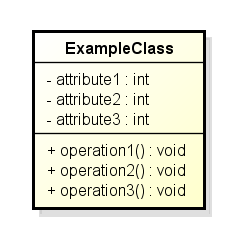
\includegraphics[scale=0.7]{./images/client/classes/example_class.png}}
				\caption{Classe - client::controller:user::FavouritesRoute}
			\end{figure}
			\begin{itemize}
				\item \textbf{Descrizione}: la classe serve a gestire l'indirizzamento e l'assegnazione di uno stato al template HTML riguardante la pagina che serve ad un utente per guardare tutti i grafici che si è salvato tra i preferiti;
				\item \textbf{Utilizzo}: viene utilizzata per reindirizzare l'utente al template HTML della pagina che permette all'utente di visualizzare i grafici che ha tra i preferiti ed assegnare al template scelto il controller opportuno per gestire i diversi compiti;
				\item \textbf{Relazioni con altre classi}:
					\begin{itemize}
						\item client::view::user::Favourites
						\item client::controller::user::FavouritesCtrl
					\end{itemize}
				\item \textbf{Attributi associati allo \$scope}: N/A
				\item \textbf{Metodi associati allo \$scope e privati}: N/A
				\item \textbf{Servizi AngularJS utilizzati}:
					\begin{itemize}
						\item \$stateProvider
					\end{itemize}
			\end{itemize}
		% subparagraph bdsm_app_client_controller_user_favouritesroute (end)


		\subparagraph{client::controller::user::FavouritesCtrl} % (fold)
		\label{subp:client_controller_user_favouritesctrl}
			\begin{figure}[htbp]
				\centering
				\centerline{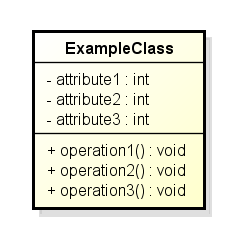
\includegraphics[scale=0.7]{./images/client/classes/example_class.png}}
				\caption{Classe - client::controller:user::FavouritesCtrl}
			\end{figure}
			\begin{itemize}
				\item \textbf{Descrizione}: la classe è il controller che serve a gestire la logica applicativa riguardante la pagina che mostra tutti i grafici che l'utente ha salvato tra i preferiti;
				\item \textbf{Utilizzo}: viene utilizzata per gestire tutti i grafici che l'utente ha salvato tra i preferiti;
				\item \textbf{Relazioni con altre classi}:
					\begin{itemize}
						\item client::model::services::RecipeService
						\item client::view::user::Favourites
						\item client::controller::user::FavouritesRoute
					\end{itemize}

				\item \textbf{Attributi associati allo \$scope}:
					\begin{itemize}
						\item \textcolor{forestgreen}{\texttt{TODO}}
							\begin{description}
								\item \textbf{Descrizione}: TODO
							\end{description}

					\end{itemize}

				\item \textbf{Metodi associati allo \$scope e privati}:
					\begin{itemize}
						\item \textcolor{forestgreen}{\texttt{TODO}}
							\begin{description}
								\item \textbf{Descrizione}: TODO
							\end{description}

					\end{itemize}

				\item \textbf{Servizi AngularJS utilizzati}:
					\begin{itemize}
						\item TODO
					\end{itemize}

			\end{itemize}
		% subparagraph client_controller_user_favouritesctrl (end)

		\subparagraph{client::controller::user::TokenConfigRoute} % (fold)
		\label{subp:bdsm_app_client_controller_user_tokenconfigroute}

			\begin{itemize}
				\item \textbf{Descrizione}: la classe serve a gestire l'indirizzamento e l'assegnazione di uno stato al template HTML riguardante la pagina che serve ad un utente per generare il token che gli consente di utilizzare i servizi REST che l'applicazione offre;
				\item \textbf{Utilizzo}: viene utilizzata per reindirizzare l'utente al template HTML della pagina che permette all'utente di generare il token necessario ad utilizzare i servizi REST pubblici ed assegnare al template scelto il controller opportuno per gestire i diversi compiti;
				\item \textbf{Relazioni con altre classi}:
					\begin{itemize}
						\item client::view::user::TokenConfig
						\item client::controller::user::TokenConfigCtrl
					\end{itemize}
				\item \textbf{Attributi associati allo \$scope}: N/A
				\item \textbf{Metodi associati allo \$scope e privati}: N/A
				\item \textbf{Servizi AngularJS utilizzati}:
					\begin{itemize}
						\item \$stateProvider
					\end{itemize}
			\end{itemize}
		% subparagraph bdsm_app_client_controller_user_tokenconfigroute (end)

		\subparagraph{client::controller::user::TokenConfigCtrl} % (fold)
		\label{subp:client_controller_user_tokenconfigctrl}
			\begin{figure}[htbp]
				\centering
				\centerline{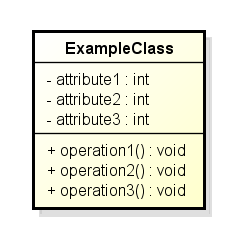
\includegraphics[scale=0.7]{./images/client/classes/example_class.png}}
				\caption{Classe - client::controller:user::TokenConfigCtrl}
			\end{figure}
			\begin{itemize}
				\item \textbf{Descrizione}: la classe è il controller che serve a gestire la logica applicativa riguardante la pagina che fornisce la possibilità ad un utente di ottenere un token da utilizzare per interrogare i servizi REST offerti;
				\item \textbf{Utilizzo}: viene utilizzata per gestire le operazioni che forniscono all'utente il token necessario ad interrogare i servizi REST offerti;
				\item \textbf{Relazioni con altre classi}:
					\begin{itemize}
						\item client::model::services::UserService
						\item client::view::user::TokenConfig
						\item client::controller::user::TokenConfigRoute
					\end{itemize}

				\item \textbf{Attributi associati allo \$scope}:
					\begin{itemize}
						\item \textcolor{forestgreen}{\texttt{TODO}}
							\begin{description}
								\item \textbf{Descrizione}: TODO
							\end{description}

					\end{itemize}

				\item \textbf{Metodi associati allo \$scope e privati}:
					\begin{itemize}
						\item \textcolor{forestgreen}{\texttt{TODO}}
							\begin{description}
								\item \textbf{Descrizione}: TODO
							\end{description}

					\end{itemize}

				\item \textbf{Servizi AngularJS utilizzati}:
					\begin{itemize}
						\item TODO
					\end{itemize}

			\end{itemize}
		% subparagraph client_controller_user_tokenconfigctrl (end)

		\subparagraph{client::controller::user::SettingsRoute} % (fold)
		\label{subp:bdsm_app_client_controller_user_settingsroute}
			\begin{figure}[htbp]
				\centering
				\centerline{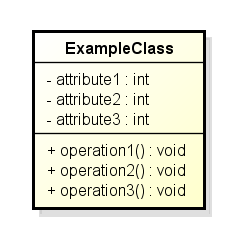
\includegraphics[scale=0.7]{./images/client/classes/example_class.png}}
				\caption{Classe - client::controller:user::SettingsRoute}
			\end{figure}
			\begin{itemize}
				\item \textbf{Descrizione}: la classe serve a gestire l'indirizzamento e l'assegnazione di uno stato al template HTML riguardante la pagina contenente le informazioni associate ad un utente e le modifiche che può effettuare su quei dati;
				\item \textbf{Utilizzo}: viene utilizzata per reindirizzare l'utente al template HTML della pagina che permette all'utente di visualizzare le impostazione del suo profilo ed assegnare al template scelto il controller opportuno per gestire i diversi compiti;
				\item \textbf{Relazioni con altre classi}:
					\begin{itemize}
						\item client::view::user::Settings
						\item client::controller::user::SettingsCtrl
					\end{itemize}
				\item \textbf{Attributi associati allo \$scope}: N/A
				\item \textbf{Metodi associati allo \$scope e privati}: N/A
				\item \textbf{Servizi AngularJS utilizzati}:
					\begin{itemize}
						\item \$stateProvider
					\end{itemize}
			\end{itemize}
		% subparagraph bdsm_app_client_controller_user_settingsroute (end)

		\subparagraph{client::controller::user::SettingsCtrl} % (fold)
		\label{subp:client_controller_user_settingsctrl}
			\begin{figure}[htbp]
				\centering
				\centerline{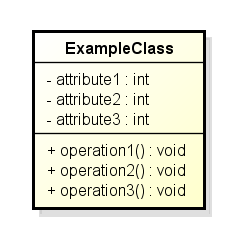
\includegraphics[scale=0.7]{./images/client/classes/example_class.png}}
				\caption{Classe - client::controller:user::SettingsCtrl}
			\end{figure}
			\begin{itemize}
				\item \textbf{Descrizione}: la classe è il controller che serve a gestire la logica applicativa riguardante la pagina che mostra le informazioni dell'utente e la possibilità di modificarle;
				\item \textbf{Utilizzo}: viene utilizzata per gestire la visualizzazione dei dati personali associati all'utente e per le operazioni di modifica;
				\item \textbf{Relazioni con altre classi}:
					\begin{itemize}
						\item client::model::data::UserModel
						\item client::view::user::Settings
						\item client::controller::user::SettingsRoute
					\end{itemize}

				\item \textbf{Attributi associati allo \$scope}:
					\begin{itemize}
						\item \textcolor{forestgreen}{\texttt{TODO}}
							\begin{description}
								\item \textbf{Descrizione}: TODO
							\end{description}

					\end{itemize}

				\item \textbf{Metodi associati allo \$scope e privati}:
					\begin{itemize}
						\item \textcolor{forestgreen}{\texttt{TODO}}
							\begin{description}
								\item \textbf{Descrizione}: TODO
							\end{description}

					\end{itemize}

				\item \textbf{Servizi AngularJS utilizzati}:
					\begin{itemize}
						\item TODO
					\end{itemize}

			\end{itemize}
		% subparagraph client_controller_user_settingsctrl (end)

		\subparagraph{client::controller::user::LogoutCtrl} % (fold)
		\label{subp:bdsm_app_client_controller_user_logoutctrl}

			\begin{itemize}
				\item \textbf{Descrizione}: la classe è il controller che serve a gestire le operazioni di logout di un utente;
				\item \textbf{Utilizzo}: viene utilizzata per distruggere la sessione attuale di un utente, attraverso la chiamata ad opportuni servizi, e il re-indirizzamento alla pagina di Login;
				\item \textbf{Relazioni con altre classi}:
					\begin{itemize}
						\item client::model::services::AuthService
						\item client::view::user::MenuMain
						\item client::controller::public::PublicRoute
					\end{itemize}
				\item \textbf{Attributi associati allo \$scope}: N/A
				\item \textbf{Metodi associati allo \$scope e privati}: N/A
			\end{itemize}
		% subparagraph bdsm_app_client_controller_user_logoutctrl (end)

% subsubsection bdsm_app_client_controller_user (end)


\subsubsection{client::controller::admin} % (fold)
\label{ssub:bdsm_app_client_controller_admin}
\begin{figure}[htbp]
	\centering
	\centerline{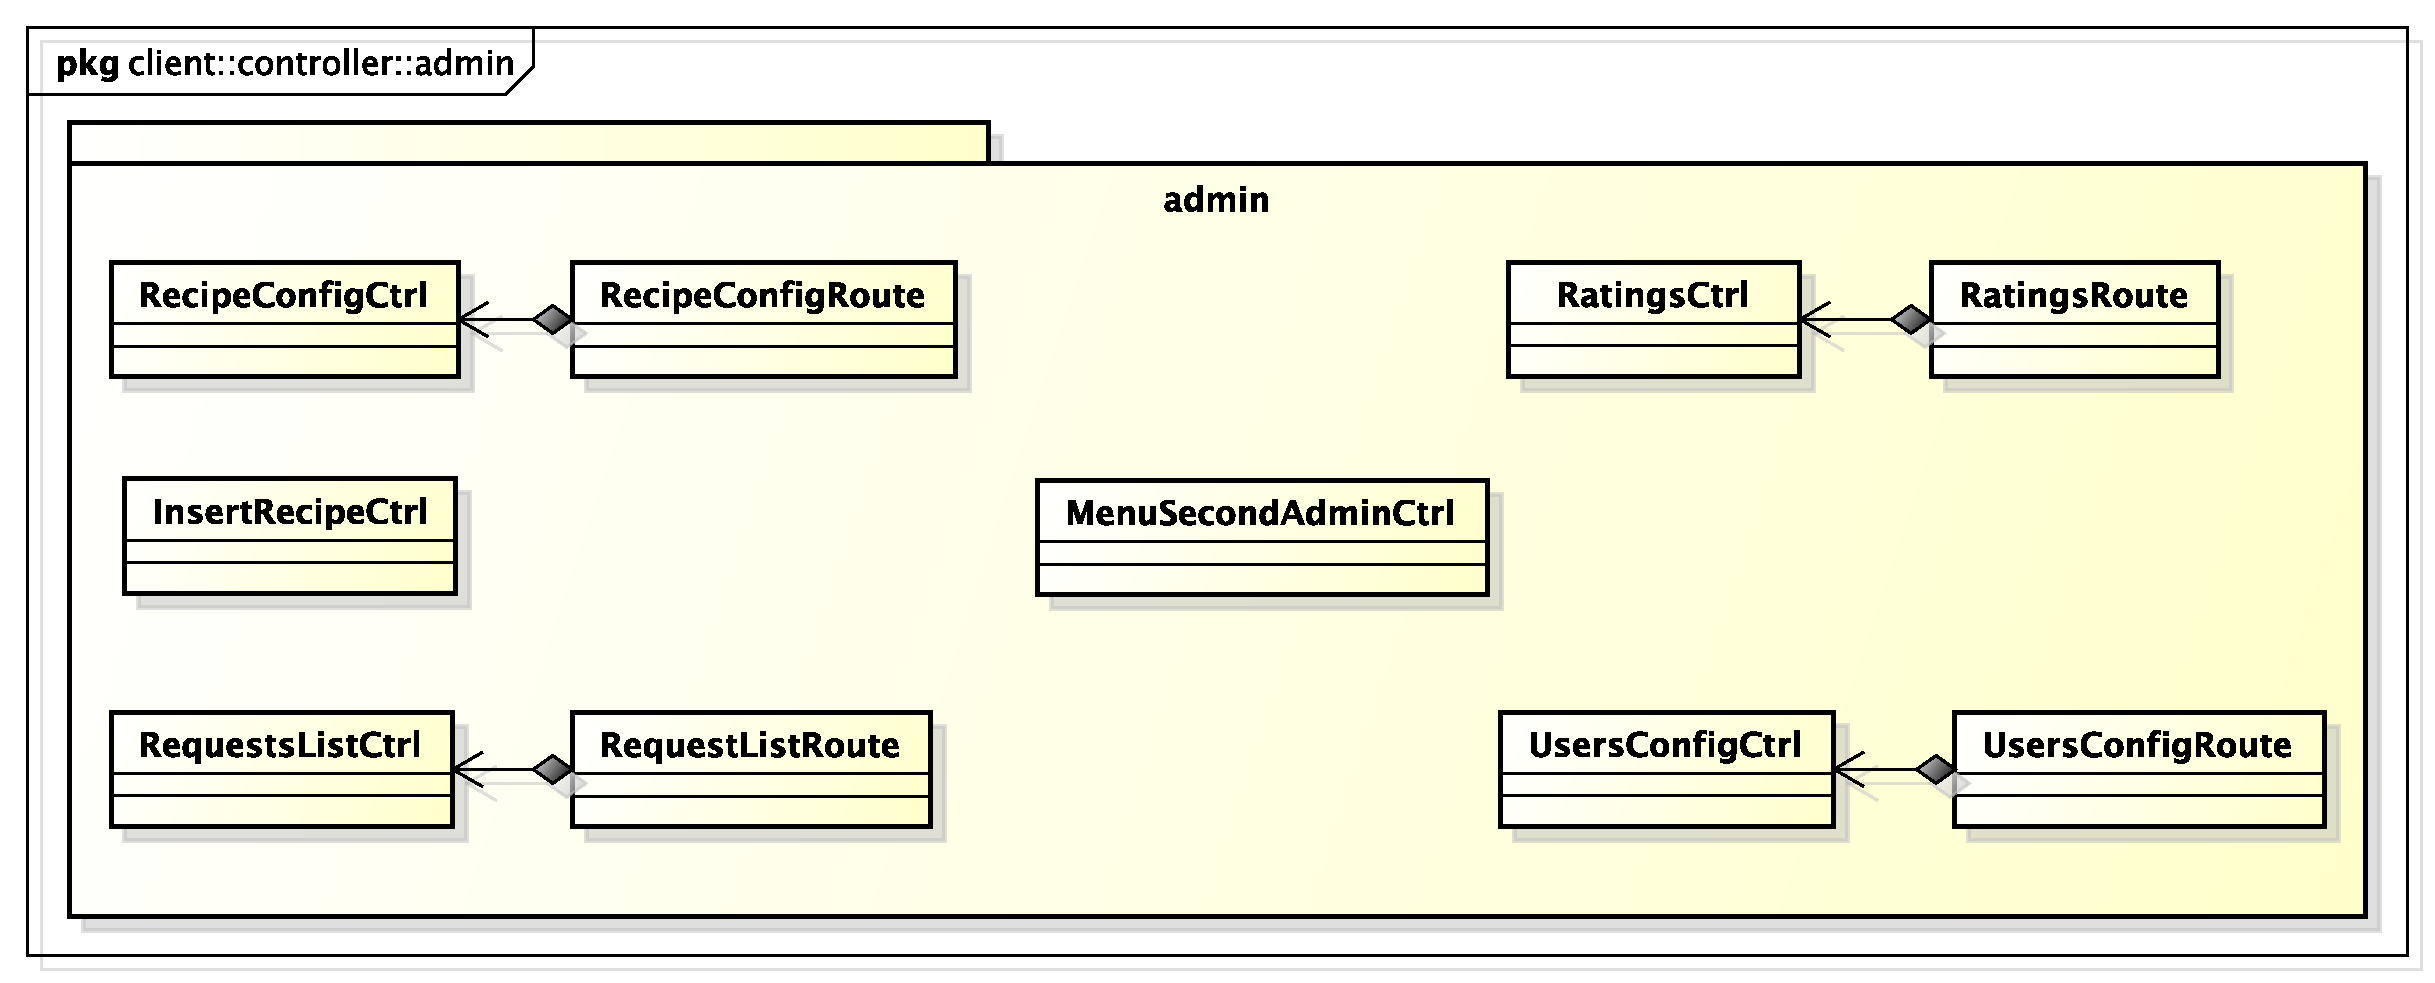
\includegraphics[scale=0.45]{./images/client/client_controller_admin.pdf}}
	\caption{Package - client::controller::admin}
\end{figure}

\begin{itemize}
	\item \textbf{Descrizione}: è il package che contiene le classi che controllano le decisioni di che pagine HTML mostrare all'amministratore e di quali operazioni poter effettuare su di esse;
	\item \textbf{Padre}: client::controller
	\item \textbf{Interazione con altri componenti}:
		\begin{itemize}
			\item client::model::admin
			\item client::view::admin
		\end{itemize}
\end{itemize}

	\paragraph{Classi} % (fold)
		\subparagraph{client::controller::admin::MenuSecondAdminCtrl} % (fold)
		\label{subp:bdsm_app_client_controller_admin_menusecondadminctrl}

			\begin{itemize}
				\item \textbf{Descrizione}: la classe è il controller che serve a gestire la logica applicativa riguardante il menu secondario dell'applicazione che ha a disposizione in più l'amministratore;
				\item \textbf{Utilizzo}: viene utilizzata per gestire i collegamenti secondari alle pagine del sistema che l'amministratore ha a disposizione per andare ad effettuare le operazioni aggiuntive a lui consentite;
				\item \textbf{Classi ereditate}:
					\begin{itemize}
						\item client::controller::user::MenuSecondCtrl. Questa ereditarietà è solo logica e non viene implementata in nessuna forma.
					\end{itemize}
				\item \textbf{Relazioni con altre classi}:
					\begin{itemize}
						\item client::view::admin::MenuSecondAdmin
						\item client::controller::admin::RecipeConfigRoute
						\item client::controller::admin::RequestListRoute
						\item client::controller::admin::RatingsRoute
						\item client::controller::admin::UserConfigRoute
					\end{itemize}
				\item \textbf{Attributi associati allo \$scope}: N/A
				\item \textbf{Metodi associati allo \$scope e privati}: N/A
			\end{itemize}
		% subparagraph bdsm_app_client_controller_admin_menusecondadminctrl (end)

		\subparagraph{client::controller::admin::RecipeConfigRoute} % (fold)
		\label{subp:bdsm_app_client_controller_admin_recipeconfigroute}

			\begin{itemize}
				\item \textbf{Descrizione}: la classe serve a gestire l'indirizzamento e l'assegnazione di uno stato al template HTML riguardante la pagina che consente di inserire una nuova Recipe nel sistema;
				\item \textbf{Utilizzo}: viene utilizzata per reindirizzare l'utente al template HTML della pagina che permette all'amministratore di andare ad inserire una nuova Recipe nel sistema ed assegnare al template scelto il controller opportuno per gestire i diversi compiti;
				\item \textbf{Relazioni con altre classi}:
					\begin{itemize}
						\item client::view::admin::RecipeConfig
						\item client::controller::admin::RecipeConfigCtrl
					\end{itemize}
				\item \textbf{Attributi associati allo \$scope}: N/A
				\item \textbf{Metodi associati allo \$scope e privati}: N/A
				\item \textbf{Servizi AngularJS utilizzati}:
					\begin{itemize}
						\item \$stateProvider
					\end{itemize}
			\end{itemize}
		% subparagraph bdsm_app_client_controller_admin_recipeconfigroute (end)

		\subparagraph{client::controller::admin::RecipeConfigCtrl} % (fold)
		\label{subp:bdsm_app_client_controller_admin_recipeconfigctrl}
			\begin{figure}[htbp]
				\centering
				\centerline{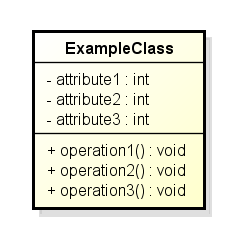
\includegraphics[scale=0.7]{./images/client/classes/example_class.png}}
				\caption{Classe - client::controller::admin::RecipeConfigCtrl}
			\end{figure}
			\begin{itemize}
				\item \textbf{Descrizione}: la classe è il controller che serve a gestire la logica applicativa riguardante la pagina che consente ad un amministratore di andare ad inserire una nuova Recipe;
				\item \textbf{Utilizzo}: viene utilizzata per gestire le operazioni che servono ad andare ad inserire una nuova Recipe;
				\item \textbf{Relazioni con altre classi}:
					\begin{itemize}
						\item client::model::data::RecipeInsertModel
						\item client::view::admin::RecipeConfig
						\item client::controller::admin::RecipeConfigRoute
					\end{itemize}

				\item \textbf{Attributi associati allo \$scope}:
					\begin{itemize}
						\item \textcolor{forestgreen}{\texttt{TODO}}
							\begin{description}
								\item \textbf{Descrizione}: TODO
							\end{description}

					\end{itemize}

				\item \textbf{Metodi associati allo \$scope e privati}:
					\begin{itemize}
						\item \textcolor{forestgreen}{\texttt{TODO}}
							\begin{description}
								\item \textbf{Descrizione}: TODO
							\end{description}

					\end{itemize}

				\item \textbf{Servizi AngularJS utilizzati}:
					\begin{itemize}
						\item TODO
					\end{itemize}

			\end{itemize}
		% subparagraph bdsm_app_client_controller_admin_recipeconfigctrl (end)

		\subparagraph{client::controller::admin::RequestListRoute} % (fold)
		\label{subp:bdsm_app_client_controller_admin_recipelistroute}

			\begin{itemize}
				\item \textbf{Descrizione}: la classe serve a gestire l'indirizzamento e l'assegnazione di uno stato al template HTML riguardante la pagina che mostra la lista di tutte le richieste di nuove Recipe;
				\item \textbf{Utilizzo}: viene utilizzata per reindirizzare l'utente al template HTML della pagina che permette all'amministratore di visualizzare la lista di tutte le richieste di nuove Recipe proposte dagli utenti ed assegnare al template scelto il controller opportuno per gestire i diversi compiti;
				\item \textbf{Relazioni con altre classi}:
					\begin{itemize}
						\item client::view::admin::RecipeList
						\item client::controller::admin::RecipeListCtrl
					\end{itemize}
				\item \textbf{Attributi associati allo \$scope}: N/A
				\item \textbf{Metodi associati allo \$scope e privati}: N/A
				\item \textbf{Servizi AngularJS utilizzati}:
					\begin{itemize}
						\item \$stateProvider
					\end{itemize}
			\end{itemize}
		% subparagraph bdsm_app_client_controller_admin_recipelistroute (end)

		\subparagraph{client::controller::admin::RequestListCtrl} % (fold)
		\label{subp:bdsm_app_client_controller_admin_requestlistctrl}
			\begin{figure}[htbp]
				\centering
				\centerline{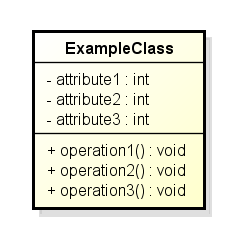
\includegraphics[scale=0.7]{./images/client/classes/example_class.png}}
				\caption{Classe - client::controller::admin::RequestListCtrl}
			\end{figure}
			\begin{itemize}
				\item \textbf{Descrizione}: la classe è il controller che serve a gestire la logica applicativa riguardante la pagina che consente ad un amministratore di visualizzare tutte le richieste di nuove Recipe inoltrate dagli utenti;
				\item \textbf{Utilizzo}: viene utilizzata per gestire le operazioni che servono ad andare a visualizzare la lista di tutte le richieste di nuove Recipe. Una volta scelta la richiesta da esaminare, l'amministratore potrà cliccare su un apposito pulsante per visualizzarne i dettagli;
				\item \textbf{Relazioni con altre classi}:
					\begin{itemize}
						\item client::model::services::RecipeAdminService
						\item client::view::admin::RecipeList
						\item client::controller::admin::RecipeListRoute
					\end{itemize}

				\item \textbf{Attributi associati allo \$scope}:
					\begin{itemize}
						\item \textcolor{forestgreen}{\texttt{+ requestList : array di oggetti JSON}}
							\begin{description}
								\item \textbf{Descrizione}: contiene la lista delle richieste di nuove Recipe proveniente dagli utenti non amministratori. Il formato degli oggetti JSON contenuti nell'array è il seguente:
								\begin{verbatim}
									{
									    idRequestRecipe: '42',
									    titleRecipe: 'Titolo della Recipe',
									    descRecipe: 'Descrizione della Recipe',
									    emailUser: 'info@mashup-unipd.it'
									}
								\end{verbatim}
							\end{description}

					\end{itemize}

				\item \textbf{Metodi associati allo \$scope e privati}:
					\begin{itemize}
						\item \textcolor{forestgreen}{\texttt{- getRequestList()}}
							\begin{description}
								\item \textbf{Descrizione}: metodo che attraverso l'invocazione del metodo \textbf{getListOfRecipesRequest()} sul servizio \textbf{recipeAdminService} riceve una promessa alla chiamata effettiva per recuperare i dati dal back-end. Quando questa sarà soddisfatta, l'attributo \textbf{requestList} verrà popolato con i dati ricevuti.
							\end{description}
						\item \textcolor{forestgreen}{\texttt{+ discardRequest(idReqRecipe)}}
							\begin{description}
								\item \textbf{Descrizione}: metodo che attraverso l'invocazione del metodo \textbf{discardRecipeRequest(idReqRecipe)} sul servizio \textbf{recipeAdminService} riceve una promessa alla chiamata effettiva per andare a rifiutare la richiesta per quella recipe. Quando questa sarà soddisfatta, verrà visualizzato un messaggio di conferma.
							\end{description}
						\item \textcolor{forestgreen}{\texttt{+ approveRequest(idReqRecipe)}}
							\begin{description}
								\item \textbf{Descrizione}: metodo che attraverso l'invocazione del metodo \textbf{approveRecipeRequest(idReqRecipe)} sul servizio \textbf{recipeAdminService} riceve una promessa alla chiamata effettiva per andare ad accettare e inserire la richiesta per quella recipe. Quando questa sarà soddisfatta, verrà visualizzato un messaggio di conferma.
							\end{description}
					\end{itemize}

				\item \textbf{Servizi AngularJS utilizzati}: N/A

			\end{itemize}
		% subparagraph bdsm_app_client_controller_admin_requestlistctrl (end)

		\subparagraph{client::controller::admin::InsertRecipeCtrl} % (fold)
		\label{subp:bdsm_app_client_controller_admin_insertctrl}
			\begin{figure}[htbp]
				\centering
				\centerline{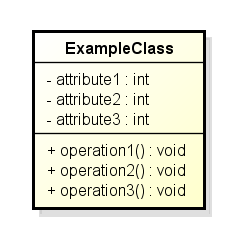
\includegraphics[scale=0.7]{./images/client/classes/example_class.png}}
				\caption{Classe - client::controller::admin::InsertRecipeCtrl}
			\end{figure}
			\begin{itemize}
				\item \textbf{Descrizione}: la classe è il controller che serve a gestire la logica applicativa riguardante il form contenente i campi necessari all'inserimento di una nuova Recipe;
				\item \textbf{Utilizzo}: viene utilizzata per gestire il form che serve per inserire una nuova Recipe nel sistema. Può essere utilizzato sia per il form di un inserimento ex novo sia per gestire i dettagli delle richieste di nuove Recipe;
				\item \textbf{Relazioni con altre classi}:
					\begin{itemize}
						\item client::model::data::RecipeInsertModel
						\item client::view::admin::Insert
						\item client::controller::admin::RecipeConfigRoute
					\end{itemize}

				\item \textbf{Attributi associati allo \$scope}:
					\begin{itemize}
						\item \textcolor{forestgreen}{\texttt{TODO}}
							\begin{description}
								\item \textbf{Descrizione}: TODO
							\end{description}
						\item \textcolor{forestgreen}{\texttt{TODO}}
							\begin{description}
								\item \textbf{Descrizione}: TODO
							\end{description}
						\item \textcolor{forestgreen}{\texttt{TODO}}
							\begin{description}
								\item \textbf{Descrizione}: TODO
							\end{description}
						\item \textcolor{forestgreen}{\texttt{TODO}}
							\begin{description}
								\item \textbf{Descrizione}: TODO
							\end{description}
						\item \textcolor{forestgreen}{\texttt{TODO}}
							\begin{description}
								\item \textbf{Descrizione}: TODO
							\end{description}
						\item \textcolor{forestgreen}{\texttt{TODO}}
							\begin{description}
								\item \textbf{Descrizione}: TODO
							\end{description}
						\item \textcolor{forestgreen}{\texttt{TODO}}
							\begin{description}
								\item \textbf{Descrizione}: TODO
							\end{description}
						\item \textcolor{forestgreen}{\texttt{TODO}}
							\begin{description}
								\item \textbf{Descrizione}: TODO
							\end{description}
						\item \textcolor{forestgreen}{\texttt{TODO}}
							\begin{description}
								\item \textbf{Descrizione}: TODO
							\end{description}
						\item \textcolor{forestgreen}{\texttt{TODO}}
							\begin{description}
								\item \textbf{Descrizione}: TODO
							\end{description}
					\end{itemize}

				\item \textbf{Metodi associati allo \$scope e privati}:
					\begin{itemize}
						\item \textcolor{forestgreen}{\texttt{TODO}}
							\begin{description}
								\item \textbf{Descrizione}: TODO
							\end{description}
						\item \textcolor{forestgreen}{\texttt{TODO}}
							\begin{description}
								\item \textbf{Descrizione}: TODO
							\end{description}
						\item \textcolor{forestgreen}{\texttt{TODO}}
							\begin{description}
								\item \textbf{Descrizione}: TODO
							\end{description}
					\end{itemize}

				\item \textbf{Servizi AngularJS utilizzati}: N/A

			\end{itemize}
		% subparagraph bdsm_app_client_controller_admin_insertctrl (end)

		\subparagraph{client::controller::admin::RatingsRoute} % (fold)
		\label{subp:bdsm_app_client_controller_admin_ratingsroute}
			\begin{figure}[htbp]
				\centering
				\centerline{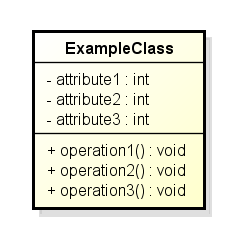
\includegraphics[scale=0.7]{./images/client/classes/example_class.png}}
				\caption{Classe - client::controller::admin::RatingsRoute}
			\end{figure}
			\begin{itemize}
				\item \textbf{Descrizione}: la classe serve a gestire l'indirizzamento e l'assegnazione di uno stato al template HTML riguardante la pagina che mostra la lista di tutte le Recipe votate con la media del valore assegnato dagli utenti;
				\item \textbf{Utilizzo}: viene utilizzata per reindirizzare l'utente al template HTML della pagina che permette all'amministratore di visualizzare la lista di tutte le Recipe votate, in ordine dalla più votata, ed assegnare al template scelto il controller opportuno per gestire i diversi compiti;
				\item \textbf{Relazioni con altre classi}:
					\begin{itemize}
						\item client::view::admin::Ratings
						\item client::controller::admin::RatingsCtrl
					\end{itemize}
				\item \textbf{Attributi associati allo \$scope}: N/A
				\item \textbf{Metodi associati allo \$scope e privati}: N/A
				\item \textbf{Servizi AngularJS utilizzati}:
					\begin{itemize}
						\item \$stateProvider
					\end{itemize}
			\end{itemize}
		% subparagraph bdsm_app_client_controller_admin_ratingsroute (end)

		\subparagraph{client::controller::admin::RatingsCtrl} % (fold)
		\label{subp:bdsm_app_client_controller_admin_ratingsctrl}
			\begin{figure}[htbp]
				\centering
				\centerline{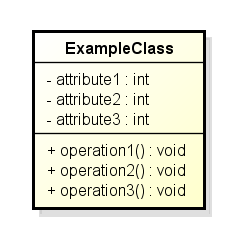
\includegraphics[scale=0.7]{./images/client/classes/example_class.png}}
				\caption{Classe - client::controller::admin::RatingsCtrl}
			\end{figure}
			\begin{itemize}
				\item \textbf{Descrizione}: la classe è il controller che serve a gestire la logica applicativa riguardante la pagina che consente ad un amministratore di visualizzare tutte le Recipe che sono state votate dagli utenti;
				\item \textbf{Utilizzo}: viene utilizzata per gestire le operazioni che servono ad andare a visualizzare la lista di tutte le Recipe che sono state votate dagli utenti, ordinandole dalla più votata alla meno;
				\item \textbf{Relazioni con altre classi}:
					\begin{itemize}
						\item client::model::services::RecipeAdminService
						\item client::view::admin::Ratings
						\item client::controller::admin::RatingsRoute
					\end{itemize}

				\item \textbf{Attributi associati allo \$scope}:
					\begin{itemize}
						\item \textcolor{forestgreen}{\texttt{TODO}}
							\begin{description}
								\item \textbf{Descrizione}: TODO
							\end{description}

					\end{itemize}

				\item \textbf{Metodi associati allo \$scope e privati}:
					\begin{itemize}
						\item \textcolor{forestgreen}{\texttt{TODO}}
							\begin{description}
								\item \textbf{Descrizione}: TODO
							\end{description}

					\end{itemize}

				\item \textbf{Servizi AngularJS utilizzati}:
					\begin{itemize}
						\item TODO
					\end{itemize}

			\end{itemize}
		% subparagraph bdsm_app_client_controller_admin_ratingsctrl (end)

		\subparagraph{client::controller::admin::UserConfigRoute} % (fold)
		\label{subp:bdsm_app_client_controller_admin_userconfigroute}

			\begin{itemize}
				\item \textbf{Descrizione}: la classe serve a gestire l'indirizzamento e l'assegnazione di uno stato al template HTML riguardante la pagina che mostra la lista degli utenti registrati al sistema;
				\item \textbf{Utilizzo}: viene utilizzata per reindirizzare l'utente al template HTML della pagina che permette all'amministratore di visualizzare la lista degli utenti registrati al sistema ed assegnare al template scelto il controller opportuno per gestire i diversi compiti;
				\item \textbf{Relazioni con altre classi}:
					\begin{itemize}
						\item client::view::admin::UserConfig
						\item client::controller::admin::UserConfigCtrl
					\end{itemize}
				\item \textbf{Attributi associati allo \$scope}: N/A
				\item \textbf{Metodi associati allo \$scope e privati}: N/A
				\item \textbf{Servizi AngularJS utilizzati}:
					\begin{itemize}
						\item \$stateProvider
					\end{itemize}
			\end{itemize}
		% subparagraph bdsm_app_client_controller_admin_userconfigroute (end)

		\subparagraph{client::controller::admin::UserConfigCtrl} % (fold)
		\label{subp:bdsm_app_client_controller_admin_userconfigctrl}
			\begin{figure}[htbp]
				\centering
				\centerline{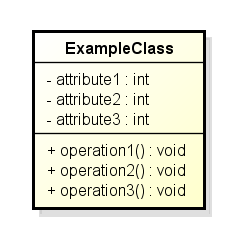
\includegraphics[scale=0.7]{./images/client/classes/example_class.png}}
				\caption{Classe - client::controller::admin::UserConfigCtrl}
			\end{figure}
			\begin{itemize}
				\item \textbf{Descrizione}: la classe è il controller che serve a gestire la logica applicativa riguardante la pagina che consente ad un amministratore di visualizzare la lista degli utenti registrati al sistema;
				\item \textbf{Utilizzo}: viene utilizzata per gestire le operazioni che servono ad andare a visualizzare la lista degli utenti registrati al sistema, potendo su di essi, andare a modificarne i permessi o a cancellare l'account;
				\item \textbf{Relazioni con altre classi}:
					\begin{itemize}
						\item client::model::services::UserAdminService
						\item client::view::admin::UserConfig
						\item client::controller::admin::UserConfigRoute
					\end{itemize}

				\item \textbf{Attributi associati allo \$scope}:
					\begin{itemize}
						\item \textcolor{forestgreen}{\texttt{usersList} : }
							\begin{description}
								\item \textbf{Descrizione}: 
							\end{description}

					\end{itemize}

				\item \textbf{Metodi associati allo \$scope e privati}:
					\begin{itemize}
						\item \textcolor{forestgreen}{\texttt{TODO}}
							\begin{description}
								\item \textbf{Descrizione}: TODO
							\end{description}

					\end{itemize}

				\item \textbf{Servizi AngularJS utilizzati}:
					\begin{itemize}
						\item TODO
					\end{itemize}

			\end{itemize}
		% subparagraph bdsm_app_client_controller_admin_userconfigctrl (end)


% subsubsection bdsm_app_client_controller_admin (end)
 \clearpage \newpage
	% END PACKAGE CONTROLLER


	% TEMPLATE PER IL PACKAGE
%	\begin{comment}
%	\subsubsection{Nome package} % (fold)
%	\label{ssub:nome_del_package}
%	[TO DO] (diagramma) \newline \newline

%	\begin{itemize}
%		\item \textbf{Descrizione}: [TO DO];
%		\item \textbf{Padre}: [TO DO] (qualora presente);
%		\item \textbf{Package contenuti}: [TO DO] (qualora presente);
%		\item \textbf{Interazione con altri componenti}: [TO DO];
%	\end{itemize}

%		\paragraph{Classi} % (fold)
%			\subparagraph{Nome package::Nome classe} % (fold)
%			\label{subp:subparagraph_name}
%				\begin{itemize}
%					\item \textbf{Descrizione}: [TO DO];
%					\item \textbf{Utilizzo}: [TO DO];
%					\item \textbf{Classi ereditate}: [TO DO];
%					\item \textbf{Relazioni con altre classi}: [TO DO].
%				\end{itemize}
			% subparagraph subparagraph_name (end)
%	\end{comment}
			% subsection nome_classe (end)

		% paragraph classi (end)
	% subsubsection nome_del_package (end)

% subsection client (end)
